\documentclass{article}
\usepackage{iclr2027_conference,times}
\input{math_commands}

\usepackage{graphicx}
\usepackage{booktabs}
\usepackage{multirow}
\usepackage{enumitem}
\usepackage{amsmath,amssymb}
\usepackage{amsthm}
\usepackage{placeins}
\usepackage[hidelinks]{hyperref}
\usepackage{xcolor}
\usepackage{url}

\newtheorem{proposition}{Proposition}
\newtheorem{corollary}{Corollary}
\theoremstyle{remark}
\newtheorem{remark}{Remark}

\renewcommand{\topfraction}{0.92}
\renewcommand{\bottomfraction}{0.92}
\renewcommand{\textfraction}{0.05}
\renewcommand{\floatpagefraction}{0.75}
\setlength{\textfloatsep}{6pt plus 2pt minus 2pt}
\setlength{\floatsep}{6pt plus 2pt minus 2pt}
\setlength{\intextsep}{6pt plus 2pt minus 2pt}
\setlength{\abovecaptionskip}{3pt}

\title{Works Where Calibrated, Fails Where Misused:\\
Auditing Small-Scale Pretraining's Seed-Noise Instruments}

\author{Anonymous\\
Affiliation\\
Address\\
\texttt{email}}

\begin{document}
\maketitle

% abstract.tex -- Rank 4 "noise-floor-trio" paper, ICLR 2027
% Revision-9: PI-approved full rewrite (~150 words; only robust transferable findings kept;
% 1.6x / 0/27 / 31-vs-37.8 / 13.5% moved to the body with their qualifiers). Numbers locked by
% review-2027/verify-scripts/check_numbers.py.

\begin{abstract}
Small-scale pretraining selects data recipes under a handful of seeds, read by three
instruments. Using only public data, we audit each where it is used: each works where
calibrated, and each fails where misused --- differently for each. The checkpoint-noise
proxy of Signal \& Noise reproduces at home but its advertised correlation is beyond
certification at realistic seed budgets for any evaluator --- a perfect proxy would read
$0.66$--$0.82$ against
$0.9$ --- and it under-reads seed noise in magnitude on the accuracy readout
(${\sim}1.6\times$ at 1B, more at smaller scales, reversed on perplexity). The init-only noise
floor is structurally unidentifiable from single-source arms at any budget; only a bundled or
crossed init$\times$order design identifies it. DataDecide's recipe ranking reproduces its
${\sim}80\%$ exactly at its recommended scale, but on the accuracy readout its separability SNR
stays at or below $1.3$ up to 60M, and at 4M the macro ranking inverts against the 1B ranking
($r = -0.56$), so seed averaging tracks the wrong ranking more faithfully. We release code, a
per-cell noise atlas (seed noise varies $2.3\times$ per recipe at 4M), and report $1{,}095$
label--config-mismatched files in PolyPythias's release.
\end{abstract}


% 01_introduction.tex -- Section 1, Introduction (compressed to <1 page for the 9-page limit)
% Red lines: no universal "never calibrated" claims; audit framed as "works where calibrated /
% fails where used". Headline numbers all remain in the main text (here and in Sections 3-7).

\section{Introduction}
\label{sec:intro}

A growing share of what the field believes about data rests on experiments that were never
meant to bear that weight: data recipes for billion-parameter runs are selected from
experiments two orders of magnitude smaller, and ablations are certified by margins of a
fraction of a percentage point, all under a handful of random seeds. Their validity hinges on a
quantity rarely measured and almost never reported: the magnitude and structure of seed-level
noise in small-scale pretraining.

The community has begun to close this gap with dedicated \emph{noise
instruments}, three of which now carry real decision weight: the checkpoint-noise proxy of
Signal \& Noise \citep{signalandnoise2025}, which reads the spread of a run's final checkpoints
as a seed-free substitute for retraining ($R^2 = 0.82$--$0.95$); the
3-seed init-only noise floor that a 2026 large-scale replication \citep{tencent2026}
operationalizes as the significance threshold for architectural claims; and
DataDecide's single-proxy recipe ranking \citep{datadecide2025}, whose ${\sim}80\%$ pairwise
accuracy at 150M is the de facto warranty for small-scale recipe selection.

\textbf{Each of these instruments works where it was calibrated. The question is whether it
works where it is used.} We audit all three against the public assets that generated them
(Section~\ref{sec:setup}). Each instrument reproduces in
its original setting and fails in the transfer setting, but the failures are of three different
kinds, and so are the verdicts. The checkpoint proxy is \emph{reproduced here, unverifiable
there}: at a 3-seed budget even a perfect proxy would typically read below the advertised
$0.9$. Source equivalence is \emph{undecidable on public evidence}: no task's interval fits a
$2\times$ band ($0/27$) --- a degrees-of-freedom statement the arm sizes force, not evidence
about the ratio --- and \emph{by construction} no enlargement of
single-source arms can identify the all-source floor.
DataDecide's recipe ranking is \emph{accurate at its recommended scale, noise-blind at the
4M--20M scales inside the proxy range in use} (RegMix fits 512 proxies of 1M parameters
\citep{liu2024regmix}; DataDecide recommends 150M \citep{datadecide2025}). These are boundary maps, not refutations.

Our findings organize around a single descriptive quantity: the \textbf{signal-to-noise ratio
(SNR) of the decision instrument} (definition: Section~\ref{sec:setup-notation}). DataDecide's
instrument operates at deconvolved SNR $\le 1.3$ at every scale up to 60M, then jumps sharply
between 60M and 90M ($1.2 \to 2.6$); at 4M--20M,
$83$--$96\%$ of its pairwise comparisons fall inside their own noise band, and at 4M
the macro-average ranking is \emph{negatively} correlated with the 1B ranking, so averaging
seeds makes decisions worse ($31.0\%$ with three seeds against $37.8\%$ with one). The
residual 150M errors are largely not repairable by seeds ($13.5\%$ [$8.3$, $57.0$]
attributable to seed noise at all). $\sigma$ itself disperses $2.3\times$ per SD across recipes
at 4M, so no measured floor transfers; and 1{,}095 released PolyPythias ``seed variant'' files
are base-model re-evaluations with \emph{exactly zero} seed variance (Appendix~\ref{app:case}).

We train nothing for the audit itself: its estimands live on the public assets themselves: whether a proxy
correlation is certifiable at the published seed budget, whether single-source arms can
identify an all-source floor, and whether a released small-scale ranking transfers to 1B are
properties of the released per-seed data -- which are therefore the complete evidence base for
these questions, not a convenience sample. A small set of self-run controls
(Appendix~\ref{app:crossed}) then supplies the two measurements no public asset contains: the
init$\times$order interaction, and the proxy's calibration at a ten-seed budget. Zero-training audits of published claims have
main-track precedent \citep{roelofs2019metaanalysis, mathur2020tangled, card2020littlepower,
polo2024tinybenchmarks}.
Contributions: (i) \textbf{a three-target audit with per-claim failure boundaries}, each
anchored in a reproduction of the original claim (Sections~\ref{sec:t1}--\ref{sec:t3}); (ii)
\textbf{a sample-complexity result and an identifiability note}: at realistic seed budgets the
proxy's advertised
correlation lies beyond any certificate's reach --- in the Fisher-$z$ limit experiment, and in
finite-sample Monte-Carlo calibration at the panel's own operating point
(Proposition~\ref{prop:t1-bound}, Appendix~\ref{app:t1-mc}) --- and single-source arms cannot
identify the all-source noise floor, a direct application of the classical variance-decomposition
fact, stated as Remark~\ref{prop:t2-nonid} because it prices what the community's floors can
and cannot mean; (iii) \textbf{the
decision-instrument SNR as a descriptive readout}, with the 4M rank inversion and a per-cell
seed-noise atlas (Sections~\ref{sec:t3}, \ref{sec:atlas}); (iv)
\textbf{prescriptions}: when cheap proxies suffice, when seeds must be measured, and what must
be declared (Section~\ref{sec:prescriptions}).

% 02_setup.tex -- Section 2, Setup (compressed; assets table + full defect text in Appendix A)
% Red lines unchanged. Notation kept in main text (Welch band + SNR definitions are load-bearing).

\section{Setup: Audited Claims, Assets, and Declared Defects}
\label{sec:setup}

We audit the three instruments as they are \emph{used} (at-a-glance map: Figure~\ref{fig:card}). Terminology (look-up table:
Table~\ref{tab:terms}, Appendix~\ref{app:setup}): a \emph{decision
instrument} is any cheap measurement whose reading stands in for an expensive one when
selecting data recipes or certifying ablations; an instrument's \emph{home setting} is the
configuration in which its advertised performance was established; and its \emph{usage
license} is the set of conditions under which its readings remain trustworthy (stated per
instrument in Sections~\ref{sec:t1}--\ref{sec:t3}). Further terms as they appear: an
\emph{arm} is one random-source condition (init-only, order-only, or bundled); a \emph{cell}
one task$\times$scale$\times$recipe point; a \emph{readout} the metric family (accuracy vs
bits-per-byte). \textbf{The checkpoint-noise proxy}: Signal \&
Noise \citep{signalandnoise2025} reports that the relative standard deviation of a run's final
checkpoints correlates with run-to-run seed noise at $R^2 = 0.82$--$0.95$ (i.e., $R \ge 0.9$),
and proposes the last-$n$-checkpoint spread as a cheap substitute for seed retraining.
\textbf{The init-only noise floor}: \citet{tencent2026} judge all 20 of their architecture claims
against a single 3-seed baseline noise floor, ``the seed-level distribution as the significance
threshold'' (their \S3.3, recommendation R5). The floor's source semantics are stated
inconsistently (\S3.3 varies ``both initialization and data-shuffle RNG'' per seed; their
appendix holds ``the shuffle seed fixed across all runs'' --- i.e.\ init-only as implemented), but either way the floor stands in
for the noise of \emph{all} random sources combined;
the auditable question is whether a single-source floor can play that role. Their per-seed
evaluations are not public as of August 2026; we audit the implemented init-only reading
(a bundled reading shifts Section~\ref{sec:t2}'s question, not its arithmetic).
\textbf{Small-scale
recipe ranking}: DataDecide \citep{datadecide2025} reports that the
ranking of 25 data recipes at a single 150M proxy scale predicts the better recipe at 1B with ${\sim}80\%$ pairwise accuracy (our reproduction: $80.2\%$ under their single-seed protocol, $82.7\%$ under 3-seed means; Section~\ref{sec:t3}); we audit the residual ${\sim}20\%$.

\paragraph{Assets and declared defects.}
All evidence comes from three public assets released with per-seed resolution:
\textbf{DataDecide} (14 sizes, 4M--1B, $\times$ 25 recipes $\times$ 3 seeds; OLMES suite
\citep{gu2025olmes} and
11-domain perplexities \citep{magnusson2024paloma}; $100$ tokens per parameter, ${\sim}5\times$Chinchilla
\citep{hoffmann2022chinchilla});
\textbf{Signal \& Noise \texttt{random\_seeds}} (20 1B runs of OLMo-2-style models
\citep{olmo2025}: 10 init-only, 9 data-order-only, 1 dense); and \textbf{PolyPythias} (50
Pythia \citep{biderman2023pythia} runs, 5 sizes $\times$ 10 seeds).
Table~\ref{tab:assets} (Appendix~\ref{app:setup}) inventories them with the defects that
constrain our methods, declared before any result.

\paragraph{Notation and estimands.}
\label{sec:setup-notation}
Throughout, $\sigma$ denotes a standard deviation of final scores across runs;
\emph{relative SD} divides by the arm mean. The proxy's \emph{calibration ratio} is
$y/x$ (true across-seed relative SD over the checkpoint-spread proxy). For
pairwise decisions we use pair-specific 95\% Welch
intervals for the difference of two 3-seed means: a pair $(i, j)$ sits inside its noise band
when $|\bar y_i - \bar y_j| < t_{0.975,\,\hat\nu_{ij}}\,\sqrt{\hat\sigma_i^2/3 +
\hat\sigma_j^2/3}$, with $\hat\nu_{ij}$ the Welch--Satterthwaite degrees of freedom. Bands within a cell are not
independent: the 300 bands of a 25-recipe cell share 25 recipe-level variance estimates, so we
read band-membership counts as descriptive tallies, not as independent tests.

\paragraph{The separability SNR.}
The
headline quantity of
Section~\ref{sec:t3} is the \emph{separability SNR}: signal $=$ the SD of the 25 recipe
means at a given proxy scale; noise $=$ the median within-recipe 3-seed SD. Because each
recipe mean itself carries seed variance $\hat\sigma_i^2/3$, the observed signal counts noise
as dispersion; we therefore also report the \emph{deconvolved} signal
$\sqrt{\max(S^2 - \overline{\hat\sigma^2}/3,\,0)}$, whose SNR uses the RMS noise
$\sqrt{\overline{\hat\sigma^2}}$ (diagnostics, robustness variants, and bootstrap intervals:
Appendix~\ref{app:t3}, Table~\ref{tab:snr-ci}). The separability SNR is target-free: it measures
separability of the proxy's readings, not correctness of its ranking (the transfer metrics carry
correctness).

% 03_t1_proxy.tex -- Section 3, checkpoint-proxy audit (compressed; tables + formal proposition
% and proofs in Appendix B)
% Numbers spot-checked: t1a_sn_replication_summary.csv (R^2 0.814/0.992 init, 0.882/0.981 order);
% t1b_summary_by_size.csv (R_log med 0.53-0.77; ceiling med 0.664-0.821; compat 0.60-0.96;
% null-indistinct 0.16-0.48); t1b_pooled_by_size.csv (1B pooled ratio 1.4256 ~ sqrt(2));
% t1c_ppl_summary_by_size.csv (detrended med_ratio_dt 750M=1.078, 1B=1.030);
% pp_t1_ratio.csv (median 1.798; blimp 70m/160m = 5.17/4.15).

\section{The Checkpoint-Noise Proxy: Reproduced Here, Unverifiable There}
\label{sec:t1}

Signal \& Noise \citep{signalandnoise2025} proposes that the spread of a training run's final
checkpoints can stand in for seed retraining: compute the relative SD of the last $n$
checkpoints of a \emph{single} run, and read it as the relative SD one would get by re-running
with new seeds. We reproduce the home result, port the proxy to its advertised use case, test it
as a magnitude substitute, and cross-check it on independent 10-seed ground truth (tables and
proofs: Appendix~\ref{app:t1}).

\paragraph{Replication in the home setting.}
\label{sec:t1-home}
On the paper's own released runs (Table~\ref{tab:t1a}) we obtain $R^2 = 0.81$/$0.99$ (init,
log/raw) and $0.88$/$0.98$ (data-order), matching two of the three published values ($0.82$
seed noise, $0.86$ data-order noise, and $0.95$ checkpoint-step noise; the range quoted in
Section~\ref{sec:intro}); the calibration
ratio $y/x$ has median $0.98$. On spaces: S\&N define noise as the \emph{raw} relative SD but
do not state the correlation's space; our log-space replication matches their values
($0.81$/$0.88$) while our raw-space replication exceeds them ($0.99$/$0.98$) --- we report both
throughout. \textbf{The claim holds in its original setting, and is
quantitatively calibrated there}; everything that follows is about transfer.

\paragraph{Porting to the advertised use case.}
\label{sec:t1-port}
The advertised use is small-scale work: many recipes, few seeds, public checkpoint grids;
Signal \& Noise itself applies the proxy exactly there, computing noise from the final five
checkpoints of the 60M--750M DataDecide models. We
port the proxy to the same asset (14 sizes $\times$ 25 recipes, $R$ across the 10 OLMES
tasks per cell; 350 cells; detail: Table~\ref{tab:t1b}). Two facts emerge.
First, the observed correlation falls short of the advertised level: per-size medians of
$R_{\log}$ range from $0.53$ to $0.77$. De-attenuated by the Monte-Carlo ceiling, however,
the medians are consistent with the advertised $0.9$ while certifying nothing:
$\hat\lambda$, the ratio of observed to perfect-proxy correlation, has median $0.93$ across
sizes, with the $1.00$ cap binding at 60M/530M and exceeded under the model-based ceiling at
90M/150M: ``consistent with $0.9$'' and ``perfect proxy'' are empirically indistinguishable at
these budgets, while certification fails regardless (Appendix~\ref{app:t1}). One caveat on
that ratio: the protocol computes the proxy on one of the same runs entering the seed
SD, so the arms' estimation errors are dependent and the ceiling is an upper bound
on the attenuation; a leave-one-seed-out variant sits slightly
lower (median $0.89$; Appendix~\ref{app:t1}). Second, and decisively, \textbf{at
this seed budget the advertised threshold is unverifiable in principle}: the ceiling above is
the distribution of $R$ for a \emph{perfect} proxy given only the sampling error of a 3-seed
SD.

The bound is structural, not a simulation artifact, and its ingredients are standard
(log-$\chi^2$ variances, errors-in-variables attenuation, Fisher-$z$ sample complexity); the
contribution is their combination for this panel. Write the log proxy SD and log seed SD per
task as $U_i = a_i + \varepsilon_i$ and $Z_i = b_i + \eta_i$, where $a_i = \log\tau_i$ is the
task's latent noise level with cross-task variance $\sigma_a^2$, and the estimation errors are
$\varepsilon_i = \tfrac12\log(\chi^2_{\nu_x}/\nu_x)$, $\eta_i = \tfrac12\log(\chi^2_{\nu_y}/\nu_y)$
from $m$ checkpoints and $n$ seeds: an errors-in-variables model with both arms noisy.

\begin{proposition}[Sample complexity of certifying a noisy proxy correlation]
\label{prop:t1-bound}
Assume iid normal arms, iid tasks, a common cross-task dispersion $\sigma_a^2$ of the latent
noise levels, and latent correlation $\lambda = \mathrm{corr}(a_i, b_i)$ between the proxy- and
seed-arm signals. Then the population correlation of the observed log-SDs is $\rho = \lambda A$
with
\[
A \;=\; \bigl[\bigl(1 + \tfrac{\psi_1(\nu_x/2)}{4\sigma_a^2}\bigr)
              \bigl(1 + \tfrac{\psi_1(\nu_y/2)}{4\sigma_a^2}\bigr)\bigr]^{-1/2} < 1 ,
\]
independent of proxy quality ($\psi_1$ trigamma; $\nu_x = m{-}1$, $\nu_y = n{-}1$). In the
Fisher-$z$ limit experiment, any level-$\alpha$ certificate of $\lambda \ge R_0$ from $k$ tasks
needs, for power $1-\beta$,
\[
k \;\ge\; 3 + \frac{(z_{1-\alpha} + z_{1-\beta})^2}
                   {\bigl[\operatorname{atanh} A - \operatorname{atanh}(A R_0)\bigr]^2}.
\]
\end{proposition}

\begin{corollary}[The 3-seed budget cannot certify $R \ge 0.9$]
\label{cor:t1-n3}
On the DataDecide panel ($k = 10$ tasks, $m \le 5$ checkpoints, $\hat\sigma_a = 0.74$), a 3-seed
arm certifying $\lambda \ge 0.9$ at $\alpha = 0.05$ has power $0.089$ even if the proxy is
perfect; certification needs $k = 266$--$1{,}516$ tasks by size (median $503$), or $n \ge 135$
seeds per arm at $m = 30$. The home budget of Signal \& Noise itself attains power only
$0.31$--$0.70$.
\end{corollary}

Proofs and the asymptotic caveats: Appendix~\ref{app:t1-proof}. No 3-seed public asset can
certify or refute the advertised threshold. The limit experiment is not doing hidden work here:
at the panel's operating point ($k{=}10$, $m{=}5$, $n{=}3$) the asymptotic certificate's
finite-sample Type-I error is $0.069$ against the nominal $0.05$, and its power against a
perfect proxy is $0.12$ (nominal $0.089$; $400{,}000$ Monte-Carlo replicates); under
equicorrelated task noise ($\rho_{\mathrm{task}}{=}0.5$) the test turns conservative and power
collapses to $0.04$ (Appendix~\ref{app:t1-mc}).

As a \emph{magnitude} substitute the picture is sharper. Pooling all 3{,}497 cells
(size $\times$ recipe $\times$ task; the 350 above are macro-only), the
calibration ratio $y/x$ has median $1.47$, or $1.61$ after the log-space small-sample
correction (median-basis; Appendix~\ref{app:t1-proof}): the proxy \emph{underestimates} true
seed noise by about $1.6\times$ (only $52.1\%$ of cells fall
within a $2\times$ band --- and that share is already evidence, because a \emph{perfect}
proxy under the same sampling noise would land only $67.9\%$ of cells inside the band),
reaching
$2.2$--$2.4\times$ at 6M/60M/150M/300M.

\paragraph{The underestimate equals the seed-semantics gap.}
\label{sec:t1-semantics}
The $1.6\times$ factor admits a second, simpler reading. The proxy was calibrated on
\emph{single-source} seed noise, while DataDecide's seeds bundle init and data order
(Section~\ref{sec:setup}). On S\&N's 1B arms, independent additivity prices bundled noise at
$\sqrt{\hat\sigma_{\mathrm{init}}^2 + \hat\sigma_{\mathrm{order}}^2}/\hat\sigma_{\mathrm{init}}
= 1.62\times$ the init-only level (median over 9 primary tasks; Table~\ref{tab:t2}) ---
equal to the proxy's apparent underestimate ($1.61$; ratio $1.00$). The 10-seed PolyPythias
cross-check shares the semantics (its seeds likewise bundle init with a pre-shuffled data
order) and brackets the same factor ($1.3$--$1.8\times$). The match of medians across different
assets is partly coincidental; the semantics reading is a hypothesis compatible with the 1B
evidence, and we flag it as such: it does not survive transfer to 20M, where the init and order
main effects are undetectable and the same proxy under-reads by $2.4$--$4.0\times$ even at a
ten-seed budget (Appendix~\ref{app:crossed}), so the $1.62\times$ factor is not defined there
at all. \textbf{The honest claim: the proxy is calibrated to whatever its training seeds varied;
at 1B that is consistent with a single source plus a predictable ${\sim}1.6\times$ semantics
gap, and at smaller scales the gap itself grows.} Whether the gap is recipe- and task-stable
is the question Section~\ref{sec:t2} shows to be undecidable on public arms.

\paragraph{Continuous metrics and an independent cross-check.}
\label{sec:t1-ppl}
On DataDecide's 11-domain perplexity tables the raw proxy fails in the \emph{opposite}
direction: it \emph{overestimates} seed noise by $2$--$7\times$ from trend contamination on
coarse grids (detrending repairs it only at ${\ge}750$M; Table~\ref{tab:t1c}); the bias
direction is metric- and grid-dependent, not a stable property one could correct for.
PolyPythias's 10-seed ground truth confirms the underestimate independently
(Appendix~\ref{app:t1-pp}): median $1.8\times$ over the 9 available cells ($1.3\times$
excluding two divergent runs at \textsc{blimp} 31m; Appendix~\ref{app:atlas}), worst
$4.2$--$5.2\times$ on saturated tasks where
step noise collapses but seed noise does not.

\paragraph{Verdict and usage license.}
\label{sec:t1-license}
\textbf{Verdict: calibrated at home; in the field, unverifiable and measuring a narrower noise
than advertised.} The proxy is real and
calibrated in its home setting; as the advertised seed-free substitute in small-scale work its
headline correlation is
unverifiable at realistic seed budgets (median ceiling $0.66$--$0.82 < 0.9$;
Corollary~\ref{cor:t1-n3}), and as a magnitude estimate it tracks the \emph{single-source}
component of seed noise --- reading low by the additivity factor on bundled-seed assets
(${\sim}1.6\times$; Section~\ref{sec:t1-semantics}) and high on coarse-grid perplexity
($2$--$7\times$; trend contamination). \textbf{License:} with a dense checkpoint grid, a
detrended
continuous metric, and explicit seed-semantics conversion, the proxy may be read
as a magnitude estimate within a $2\times$ band in the median; we observe the detrending repair
at the two largest scales only (750M, itself budget-truncated, and 1B) --- two points, not a
threshold; and even inside the license $37$--$46\%$ of cells fall outside the band, with the
repair non-monotone in scale (Appendix~\ref{app:t1-ppl}). In all other regimes (few-seed comparisons,
accuracy metrics at small scale, saturated tasks), seed noise must be measured.

% 04_t2_source_equiv.tex -- Section 4, source-equivalence audit (compressed to ~1 page
% revision-9; 27-task table, power table, sensitivity table, proofs in Appendix C)
% RED LINE 1 preserved: the x1.62 factor is reported ONLY as a sensitivity result under an
% additivity assumption, juxtaposed with the 1.06/1.19 empirical check; never actionable.

\section{Source Equivalence: Undecidable on the Richest Public Arms}
\label{sec:t2}

As implemented, the \citet{tencent2026} floor is single-source
(Section~\ref{sec:setup}), so its use as the significance threshold prices all-source noise from
one source. Because \citet{tencent2026}'s per-seed evaluations are not public, what we audit is
the \emph{practice} --- a single-source floor read as an all-source threshold --- on the richest
public arms with both sources present (S\&N's 10 init-only and 9 data-order-only 1B runs); the
verdict binds the practice wherever it is used. We assess equivalence against a
$[0.5, 2]$ band on $\sigma_{\mathrm{init}}/\sigma_{\mathrm{order}}$ with F and bootstrap
intervals (per-task table: Appendix~\ref{app:t2}) --- a conventional parity tolerance,
descriptive rather than a validity threshold (parity is neither necessary nor sufficient for
the floor's validity). Two questions must be kept
apart: an \emph{empirical} one --- are the two sources comparable in magnitude --- which more
single-source runs could answer (Table~\ref{tab:t2power}), and a \emph{structural} one ---
does either marginal arm identify the all-source floor at all --- which they cannot, at any
arm size (Remark~\ref{prop:t2-nonid}). The $0/27$ below bears on the first, as a power
statement; the second stands by construction.

The median ratio is $0.79$ on primary tasks and $1.17$ on bpb (point estimates, exploratory
only: Appendix~\ref{app:t2}). Not one of the 27 tasks has a CI inside the $2\times$ band
($0/9$ primary, $0/18$ bpb under the analytic F intervals; $2/27$ under bootstrap) --- a
precision statement the degrees of freedom force, not evidence about the ratio (even at $n=10$
per arm the F interval's half-width is $4.03\times$ on the variance-ratio scale;
Table~\ref{tab:t2power}). The structural point is separate: writing a run's final score as
$f(i,d) = \mu + a(i) + b(d) + c(i,d)$, the init arm identifies the law of $\mu + a(I)$, the
order arm that of $\mu + b(D)$, and the interaction $c$ lives off both arm lines at \emph{any}
arm size (proofs: Appendix~\ref{app:t2-proof}). The remark below prices this classical
variance-decomposition fact \citep{searle1992variance} at the public arm sizes --- stated because it bounds what single-source floors can
mean, not because it is new.

\begin{remark}[Non-identifiability of the all-source floor]
\label{prop:t2-nonid}
Let the two arm laws have variances $\sigma_i^2, \sigma_o^2 > 0$ and atomless source
distributions (a two-point example in Appendix~\ref{app:t2-proof} witnesses the same
phenomenon for a discrete law). Then
\emph{(i) observational equivalence}: data-generating processes with identical arm laws realize
all-source variances $\sigma_{\mathrm{all}}^2$ of $\sigma_i^2$ \emph{(the init-only floor is
exact)} and $\sigma_i^2 + \sigma_o^2$ \emph{(independent additivity)} alike.
\emph{(ii) one-sided under no cancellation}: if the interaction covaries with neither main
effect, $\rho = \sigma_{\mathrm{all}}/\sigma_i \ge \sqrt{1 + \sigma_o^2/\sigma_i^2}$, and that
no-cancellation premise is itself untestable from these arms.
\end{remark}

So at every public arm size the $27$ tasks' arm laws are compatible with both $\rho = 1$
\emph{(the floor is exact)} and independent additivity alike, and no single-source data
exclude either.

Read under \citet{tencent2026}'s bundled \S3.3 semantics, the empirical check would need a
bundled arm the public record lacks; the structural answer is unchanged
(Remark~\ref{prop:t2-nonid}).

\paragraph{Verdict.}
\label{sec:t2-verdict}
\textbf{Undecidable on public evidence, by construction.} This binds the
\emph{practice} --- a single-source floor read as an all-source threshold --- not
\citet{tencent2026}'s own implementation, whose per-seed data are not public. Under a
conditional reading --- the target experiment holding the data order fixed and randomizing
init only --- the same floor estimates a narrower estimand and is not thereby invalid.
(The two sources are of comparable magnitude at 1B, so an init-only floor is not orders of
magnitude off: under independent additivity the understatement factor is $1.3$--$1.6$, a
model-based sensitivity estimate the available cross-check cannot confirm.)
\textbf{The headline
is the design consequence}: what identifies the all-source floor is a bundled arm or a crossed
init$\times$order design (Appendix~\ref{app:crossed}), not more single-source runs.

% 05_t3_decision_snr.tex -- Section 5, decision replay + SNR headline (compressed; full replay
% table and HME table in Appendix D)
% RED LINE 4 honored: 54-59%/82% stated descriptively ("land on pairs that a re-draw of seeds can
% flip"), never "caused by seed noise". RED LINE 2 honored: SNR framed as audit of DataDecide's
% published decision procedure; non-independence of pairs declared.
% Spot checks: t3_decision_replay.csv 150M macro row (acc 0.8267/0.8022, 52 err, 28 unstable).

\section{Decision Replay: 80\% Correct at 150M, Noise-Limited Below 90M}
\label{sec:t3}

DataDecide's headline number---rankings at a single 150M proxy scale pick the better 1B data
recipe with ${\sim}80\%$ pairwise accuracy---is the de facto warranty for small-scale recipe
selection. That number averages three \emph{per-seed} decision attempts; their Figure~1
(right) draws the envelope against compute. Their text names the confound our model resolves
(``it is difficult to distinguish evaluation variance from true crossovers''). We audit both readings of the instrument on the
released tables: target $=$ each
recipe's 1B score; prediction $=$ proxy-scale final scores, under single seeds (their
protocol) and 3-seed means (our variant); decisions $=$ all $\binom{25}{2} = 300$ unordered
pairwise comparisons, per task and per scale (Appendix~\ref{app:t3}, Table~\ref{tab:t3}).

\paragraph{The claim reproduces exactly.}
\label{sec:t3-repro}
At 150M, macro-average pairwise accuracy is $80.2\%$ under their single-seed protocol: the
published ${\sim}80\%$ to the digit (Figure~\ref{fig:t3}, left, the final-checkpoint slice of
that envelope). With 3-seed means it reads $82.7\%$. What the envelope does not show: the
per-scale noise budget (Table~\ref{tab:snr}), the noise-band coverage, and the behaviour off
the recommended scale, where its own curve already dips below chance without comment (the 4M
inversion below).

\paragraph{What the residual 20\% is made of.}
\label{sec:t3-decomp}
We call a comparison \emph{seed-unstable} if the pairwise decision is not invariant within
the released seeds: $54\%$ of the 52 macro errors at 150M land on such pairs ($59\%$ pooled
over 90M--750M; $82\%$ at task level), a ${\sim}2\times$ enrichment over the $26$--$31\%$ base
rate. The count reports where errors land, not what caused them: the classifier judges
\emph{single-seed} decisions (DataDecide's own protocol; our variant averages three), and the
same three seeds define both instability and the target ranking.

A hierarchical measurement-error model makes both caveats quantitative (specification and
per-scale table: Appendix~\ref{app:t3-hme}, Table~\ref{tab:hme}; empirical
Bayes, reproducing the replay itself: $52.4$ expected errors at 150M macro versus $52$
observed). (i) An independent re-draw of the three seeds flips the 3-seed-mean pairwise decision
with probability $7.2\%$ on average at 150M macro. (ii) $13.5\%$ [$8.3$, $57.0$] of the
expected residual errors are attributable to seed noise at all; the remainder is latent
proxy--target discordance ($\hat\rho = 0.79$ at 150M macro), which no amount of seed averaging
can remove, though the interval does not exclude a majority seed-noise share.
(iii) The decisions taken forfeit an expected $10.9\%$ of the total
pairwise target signal. The realized argmax pick at 150M --- the usage DataDecide recommends ---
is \texttt{DCLM-Baseline (QC FW 3\%)}, which ranks 21st of 25 at 1B ($-4.6$
macro points below the best), while the top-3 picks at 150M rank 21st/11th/3rd at 1B; a
noiseless ranking would still forfeit $-3.9$. The same recipe is the single influential outlier
in the 150M attribution (dropping it raises the seed-noise share from $0.13$ to $0.29$;
Section~\ref{sec:limitations}): one QC-filtered variant over-performs at small scale and
reverts at 1B. Read as top-$k$ regret --- the practitioner's metric --- the realized top-1 pick
forfeits $5.9$ macro points at 4M (1B rank 24/25) and $4.7$ at 150M (21/25), with
seed-resampled 95\% intervals excluding zero throughout ([1.7, 6.8] and [4.3, 5.3] points). At the point estimates,
the instrument's ceiling is latent, seed noise the smaller term. The model also re-reads
the descriptive share: the
classifier's $54\%$ corresponds to a true flippable share of $29\%$ [$16$, $47$]
(Appendix~\ref{app:t3-hme}).

\paragraph{The headline: the decision instrument's signal-to-noise ratio.}
\label{sec:t3-snr}
Accuracy percentages bury the operational question: \emph{at a given proxy scale, how large is
the signal to rank, relative to the noise given?} Table~\ref{tab:snr}
computes, per scale, the decision-instrument SNR
(Section~\ref{sec:setup-notation}) and the share of the 300 recipe pairs whose mean
difference falls inside its pair-specific 95\% Welch noise band (a $z$ approximation understates
the shares: $47$--$89\%$ vs.\ $83$--$96\%$ at 4--20M).

\begin{table}[!tbp]
\centering
% TABLE-SNR: revision-3 version. Observed columns = pre-revision definition (bridge);
% deconvolved columns from review-verify/w1_v2_final.csv (w1_v2_final.py, B=2000 recipe-cluster
% bootstrap); Welch column unchanged (MF-3 recomputation, CHANGES-REVISION-1.md); z column dropped.
\caption{\textbf{SNR of the DataDecide decision instrument, by proxy scale.} Observed columns as defined in Section~\ref{sec:setup-notation}; the deconvolved columns
remove the seed variance each recipe mean carries (diagnostics, untruncated differences,
median-based variants, and bootstrap intervals: Table~\ref{tab:snr-ci}). $^*$Truncates at zero
at 10M: the across-recipe signal there is indistinguishable from seed noise (95\% upper limit
on the SNR $0.43$). \emph{Inside Welch band}
$=$ share of the 300 recipe pairs inside the pair-specific 95\% Welch band for two 3-seed
means; at $n{=}3$ the band is wide, so a high share prices the
instrument's power, not evidence that recipes are equal (Section~\ref{sec:t2}). The 6M/8M/16M
noise medians coincide only at the displayed precision (full precision
$0.004059$/$0.004060$/$0.004062$; mechanism: Appendix~\ref{app:atlas}). Note the two SNR
columns aggregate noise differently --- the observed column divides by the median
within-recipe SD, the deconvolved column by the RMS noise
(Section~\ref{sec:setup-notation}) --- so the two are not row-by-row comparable.}
\label{tab:snr}
\scriptsize
\setlength{\tabcolsep}{3pt}
\renewcommand{\arraystretch}{0.80}
\begin{tabular}{@{}lcccccc@{}}
\toprule
proxy scale & signal (obs.) & signal (deconv.) & noise & SNR (obs.) & SNR (deconv.) &
inside Welch band \\
\midrule
4M   & 0.00590 & 0.00270 & 0.00874 & 0.67 & 0.30 & 93.7\% \\
6M   & 0.00573 & 0.00422 & 0.00406 & 1.41 & 0.63 & 83.7\% \\
8M   & 0.00441 & 0.00220 & 0.00406 & 1.08 & 0.33 & 95.7\% \\
10M  & 0.00385 & 0$^*$   & 0.00386 & 1.00 & 0.00 & 93.0\% \\
14M  & 0.00543 & 0.00246 & 0.00709 & 0.77 & 0.29 & 95.7\% \\
16M  & 0.00681 & 0.00530 & 0.00406 & 1.68 & 0.72 & 83.0\% \\
20M  & 0.00693 & 0.00555 & 0.00649 & 1.07 & 0.77 & 86.7\% \\
60M  & 0.01142 & 0.01034 & 0.00766 & 1.49 & 1.23 & 72.7\% \\
90M  & 0.01687 & 0.01647 & 0.00469 & 3.60 & 2.61 & 47.0\% \\
150M & 0.02035 & 0.02003 & 0.00555 & 3.67 & 3.18 & 38.7\% \\
300M & 0.02296 & 0.02266 & 0.00561 & 4.09 & 3.57 & 36.7\% \\
530M & 0.02347 & 0.02304 & 0.00686 & 3.42 & 2.98 & 39.3\% \\
750M & 0.02182 & 0.02127 & 0.00414 & 5.26 & 2.52 & 46.7\% \\
1B   & 0.02057 & 0.02030 & 0.00355 & 5.79 & 3.52 & 33.0\% \\
\bottomrule
\end{tabular}
\end{table}

The gradient is stark, and it is not smooth (Table~\ref{tab:snr}, Figure~\ref{fig:snr}): the
deconvolved SNR, which removes the seed noise
counted inside the raw signal (Section~\ref{sec:setup-notation}), reads $0.30$ at
4M, $0.77$ at 20M, $1.23$ at 60M, then jumps to $2.61$ at 90M (paired-bootstrap 95\% CI on the
ratio $[1.6, 3.0]$; 150M: $3.18$; 1B: $3.52$); the
indistinguishable share falls from $94\%$ at 4M to $33\%$ at 1B. At 10M the deconvolved signal
truncates at zero ($95\%$ upper limit $0.43$; robust to trimming the two highest-noise recipes,
Table~\ref{tab:snr-ci}); the observed $58.0\%$ there is what such an instrument delivers: the
fitted model's latent signal variance is itself zero at 10M, and simulated datasets score $50\%$
on average (95\% range $[37\%, 64\%]$), containing the observed value. This is a statement
about the macro readout, not about the tasks: read per task, the same 10M models decide
$64.0\%$ of pairs correctly --- macro aggregation cancels task-level signals that point in
different recipe directions. \textbf{At every scale up to 60M the instrument operates at
deconvolved SNR $\le 1.3$ (upper 95\% limits below $1.7$), and at the 4M--20M scales inside
the proxy range in use, more than four-fifths of all pairwise comparisons fall
inside their own noise band.} On this asset and readout, the envelope's lower edge is crossed
between 60M and 90M --- the jump survives leave-one-recipe-out at the macro level (60M SNR
$\in [1.13, 1.35]$, 90M $\in [2.38, 2.81]$ over all 25 drops) and appears in 6 of 10
task-level readouts --- well below the recommended 150M. Nor is the SNR readout tautological
with accuracy: read per task, the per-task deconvolved SNR predicts the per-task pairwise
accuracy out of sample --- Spearman $+0.39$ at 4M rising monotonically to $+0.90$ at 150M and
$+0.92$ at 530M ($p<0.001$ at both) across the ten held-out tasks.

\paragraph{At the smallest scale, aggregation hurts.}
\label{sec:t3-inversion}
At 4M the macro decision accuracy is \emph{below the coin flip}, and seed averaging makes it
worse: $31.0\%$ correct with 3-seed means against $37.8\%$ with single seeds
(Table~\ref{tab:t3}). The mechanism is visible in the rankings themselves: the 4M macro ranking
of the 25 recipes correlates with the 1B ranking at $r = -0.56$ (Pearson, $p = 0.004$; Spearman
$-0.52$; leave-one-recipe-out $[-0.67, -0.50]$), and the correlation climbs monotonically to
$+0.91$ at 530M. The inversion is a property of the macro-average readout, not of any single
task: per-task 4M--1B correlations range from $-0.27$ (winogrande) to $+0.88$ (arc\_easy) and
are positive on 5 of the 10 tasks, while the macro average flips negative. This is an
aggregation effect: the tasks carry different shares of the cross-recipe variance at the two
scales. It is not an artifact of the aggregation rule, either: the correlation stays
non-positive under median, z-score, rank, and min-max readouts ($-0.36$ to $-0.55$) and
negative under 9 of 10 leave-one-task-out drops with the mean readout (10 of 10 for every
other readout; worst case $+0.11$). Nor is it an artifact of
recipe relatedness: a cluster bootstrap over the 10 recipe families gives 95\% CI
$[-0.82, -0.16]$ for the 4M macro correlation ($P(r{>}0) = 0.001$). And it is not one task's
residual signal either: per-task 4M accuracies sit on both sides of chance
($34$--$91\%$; Appendix~\ref{app:t3}). It also reconciles Table~\ref{tab:t3}'s 4M row with itself (task-level $54.9\%$ above
chance; macro $31.0\%$ below), and it survives the readout change: under a bpb proxy
at 4M (S\&N's re-evaluation; single-seed 1B target) the correlation is $-0.35$, weaker but
still negative (leave-one-recipe-out $[-0.40, -0.29]$). At 4M the small-scale ordering is
negatively informative about the target
ordering: single-seed noise partially masks the inversion by pushing decisions toward chance,
while 3-seed averaging tracks the wrong ranking more faithfully; averaging pays only when the
latent proxy ranking is positively informative about the target, and at SNR $\le 1$ that sign
is unknown. Such inversions have an independent, documented cause: repetition rates
shift with the training budget \citep{zhou2026repetition}.

% FIG-F4 and FIG-F5 live here (redrawn: make_t123_pp.py, make_f5_snr.py); side-by-side float
% to fit the 9-page limit (both figures stay in the main text).
\begin{figure}[!tbp]
\centering
\includegraphics[width=0.58\linewidth,height=0.17\textheight,keepaspectratio]{figures/F5_snr_headline.pdf}
% FIG-F5: SNR vs scale + indistinguishable-pair share; numbers = MF-3 Welch recomputation.
\caption{\textbf{The decision instrument's SNR.} SNR (left axis) and share of pairs inside
their Welch band (right axis) by proxy scale; shading ends at 60M. The series shown is the
observed variant; Table~\ref{tab:snr} carries the deconvolved correction. (Replay panels:
Figure~\ref{fig:t3}, Appendix~\ref{app:t3}.)}
\label{fig:snr}
\end{figure}

\paragraph{Estimand, dependence, verdict.}
\label{sec:t3-estimand}
This SNR audits one published decision procedure on its own candidate set (these 25 recipes,
one proxy scale); it is not a transferable constant of small-scale
pretraining. The 300 pairs share 25 recipes, so pair counts are descriptive coverage, with
inferential weight carried by the per-scale aggregates. \textbf{Verdict: accurate at its recommended scale, with a mapped operating
envelope}: our replication \emph{confirms} the published claim at 150M, and we add the SNR
gradient delimiting where the instrument can see plus the 4M inversion where aggregation
backfires.


\section{The $\sigma$ Atlas: Seed Noise Is Not Recipe-Invariant}
\label{sec:atlas}

Behind all three audits sits one quantity: the per-cell seed noise $\sigma$, released as an
atlas (14 sizes $\times$ 25 recipes $\times$ 11 domains, the 3-seed SD of final log-perplexity
per cell, 3{,}850 cells; Table~\ref{tab:sigma}, Appendix~\ref{app:atlas}). Two
structural conclusions follow.

First, the floor is far from zero where small-scale recipe work is done: median $\sigma$ is
$0.008$--$0.029$ nat over 4M--20M (the 20M elevation: Appendix~\ref{app:atlas}), and rank-adjacent recipes sit a median $0.5$--$1.9$ seed SDs apart on the log-ppl readout over 4M--20M (quantiles: Appendix~\ref{app:atlas}). The
floor then falls with scale ($0.0043$ nat median at 150M).

Second, $\sigma$ is not a constant one could measure once and export. Varying \emph{only the
data recipe} at fixed size and domain disperses $\sigma$ well beyond the $\chi^2_2$ sampling
law: at 4M a true spread of $1.5\times$ per SD in the median domain
and $2.29\times$ in the most dispersed one (C4-en; 95\% recipe bootstrap $[1.47, 3.06]$;
homogeneity test $p = 0.005$), $1.78\times$ at 20M
(carried by one recipe), and $1.65\times$ at 150M (not significant). The 1B row exercises the
null side: observed variance falls \emph{below} the sampling floor and the estimator
returns exactly $1.00\times$ (per-domain robustness: Appendix~\ref{app:atlas}).
\textbf{$\sigma$ is not a transferable constant; it is a function of the recipe} --- a floor
measured on one rig cannot be a community threshold (at $\pm 1$ SD the 4M recipe dependence
alone spans $5.3\times$).

PolyPythias anchors the atlas in absolute accuracy units with 10 seeds per cell
(Appendix~\ref{app:atlas}).
All $\sigma$ values describe the released assets' regime (published recipe families,
${\sim}5\times$Chinchilla budgets); other budgets or recipes require remeasurement.

% 08_prescriptions.tex -- Section 8, prescriptions (compressed; metric-panel table to Appendix G)
% RED LINE 2 honored: no "switching metrics beats adding seeds"; panel reported as observation.

\section{Prescriptions: When Proxies Suffice, When Seeds Must Be Measured}
\label{sec:prescriptions}

The audits converge on four positive rules.

\begin{enumerate}[leftmargin=1.6em,itemsep=1pt,topsep=2pt]
\item \textbf{The checkpoint proxy has a license, and the license has edges.}
The proxy may be read as a magnitude estimate, within a $2\times$ band in the median, only
with all of: a dense final checkpoint grid; a detrended continuous metric;
and an explicit seed-semantics conversion --- on bundled-seed setups the proxy reads low by
a factor consistent with the single-source/bundled semantics gap (${\sim}1.6\times$ on the public
1B arms --- a single-asset observation; $2.4$--$4.0\times$ at our 20M control, a
single-point observation on a different recipe and re-implemented stack; the semantics
reading itself is a hypothesis that does not survive transfer to 20M,
Section~\ref{sec:t1-semantics}),
whose stability across recipes is undecidable on public evidence: the conversion factor must
be re-measured where it is used
(Sections~\ref{sec:t1-semantics}, \ref{sec:t2}). The detrending repair appears at the two
largest scales only --- two points, not a threshold --- and even inside the license
$37$--$46\%$ of cells fall outside the band. Outside
these edges, seed noise must be
measured; no new correlation claim can rescue it (Section~\ref{sec:t1-port}).
\item \textbf{Reported noise must declare its source semantics and its recipe.}
``Seed noise'' is ambiguous between init-only, order-only, and bundled sources
(Section~\ref{sec:t2}), and the
magnitude is recipe-dependent at fixed scale (Section~\ref{sec:atlas}). A reported $\sigma$
without a source and a recipe is not a number others can use.
\item \textbf{Compute the SNR and the decidable share before deciding.}
Before ranking candidates at
a proxy scale, run the reference implementation on the per-candidate, per-seed final
scores (Appendix~\ref{app:t3} lists it verbatim; it reproduces Table~\ref{tab:snr} to the
digit), and report the \emph{decidable share}: the fraction of pairs whose difference clears
its pair-specific Welch band after multiplicity control. The 300 pairs share 25 recipes, so
the control must be dependence-robust --- Benjamini--Yekutieli \citep{benjamini2001by} or a
max-$T$ bootstrap --- with Benjamini--Hochberg \citep{benjamini1995controlling} kept as the
generous reference (Table~\ref{tab:decidable}). On this panel's
macro readout the share is essentially zero at every scale ${\le}60$M under every rule (the
only exceptions: $1.3\%$ at 6M under BH and one pair at 16M under max-$T$) ---
below 60M the honest output is abstention, which avoids the 4M catastrophe outright
(the 4M argmax pick forfeits $5.9$ macro points at 1B); at ${\ge}90$M the share is
rule-dependent ($37$--$62\%$ under BH, $1$--$16\%$ under the dependence-robust rules), so
report it under a dependence-valid rule, not BH alone. (The variance model matters more than
the multiplicity rule at the boundary: with the variance pooled across recipes, df $= 50$,
the 4M/10M zero survives (16M/20M read $4$/$7\%$ under pooled BH, $0$ under BY) but 60M reads
$19$--$34\%$;
Table~\ref{tab:decidable}.) Where
pairs are decidable, decisions
restricted to them are strictly more accurate on this panel ($88$--$96\%$ vs $80$--$88\%$
unrestricted, 90M--530M; Appendix~\ref{app:t3}). The share is
\emph{target-free}: it prices resolvability, not correctness --- at 4M more seeds would merely
resolve more pairs of an inverted ranking ($56\%$ at $n{=}30$), so separability is necessary,
not sufficient (Section~\ref{sec:t3-inversion}). The empirical mapping (task-level, 80 cells;
Spearman $+0.89$ pooled across scales, $+0.39$ within 4M alone): separability SNR $0.5$--$1 \to 63\%$ pairwise accuracy, rising to
$88$--$93\%$ at SNR ${\ge}2.5$ (full bin table and the per-scale indistinguishability blocks:
Appendix~\ref{app:t3}.) The seed answer has a price --- and it is not the first lever: at comparable token budget ($15$B vs $18$B tokens),
moving up in scale beats adding seeds on this panel ($80\%$ at 150M$\times$1 seed vs $76\%$
at 60M$\times$3), and also at comparable FLOPs ($78.2\%$ at 90M$\times$1 seed
vs $76.3\%$ at 60M$\times$3 seeds --- $0.75\times$ the FLOPs by $6ND$), so \emph{scale first};
where the scale is pinned, the decidable share
leaves zero at $n{=}4$ seeds and passes $50\%$ at $n{=}8$ at 60M, while at 4M even $n{=}30$
buys only $56\%$ (Appendix~\ref{app:t3}).
\item \textbf{At the released 3-seed budget, sub-$1\sigma$ gaps are not resolved decisions.}
At 14m--31m, $1\sigma$ of seed noise is already $0.5$--$1$ accuracy point on saturated
benchmarks; at 4--20M in log-ppl, $0.008$--$0.029$ nat
(Section~\ref{sec:atlas}). Smaller margins are noise-band differences; the $1\sigma$ rule is the necessary screen,
not the sufficient test --- significance needs the pair-specific band: at $n = 3$ the 95\%
Welch band is $2.0$--$2.5$ times the larger within-recipe SD
(Welch df $4$ down to $2$ as the variance imbalance grows).
\end{enumerate}

(One further regularity, scoped plainly in Appendix~\ref{app:metric-panel}: the readout metric
alone moves the instrument's SNR by a median $1.8$--$4.0\times$ in bpb's favor, $2.2$--$5.8\times$
at ${\le}20$M after deconvolution.)

\section{Related Work}
\label{sec:related}

Run-to-run variability is well documented \citep{nondeterminism2021, latentstate2023,
picard2021seed, reimers2017reporting, bouthillier2019unreproducible}; error bars on LLM
evaluations, and the small-$n$ statistics beneath them, are quantified and faulted by
\citet{miller2024errorbars, madaan2024variance, bowyer2025clt}; and the significance-testing
and seed-budget guidance literature \citep{dror2018hitchhiker, dodge2019showyourwork,
colas2018howmany} is what Section~\ref{sec:prescriptions} prices at pretraining scale. \citet{nityasya2023debt} call the cost of
under-measured claims \emph{scientific debt}; rliable \citep{agarwal2021rliable} is our
closest methodological kin. Where this literature measures instability, we audit the
instruments built to \emph{price} it --- and supply the magnitudes and regime boundaries such
error bars need.

Three works are closest in method. \citet{dodge2020finetuning} introduce the crossed
init$\times$order design our public assets lack, for fine-tuning; we add why the design is
\emph{necessary} --- the interaction term is unidentified from single-source arms at any
budget (Section~\ref{sec:t2}) --- and a crossed grid trained at pretraining scale (20M,
Appendix~\ref{app:crossed}). \citet{bouthillier2021variance} account for variance in
benchmark comparisons by measuring both seeds and bootstrap resamples
\citep{dehghani2021lottery}; we add the per-cell magnitudes such accounting needs (the
$\sigma$ atlas) and the finding that the floor is recipe-dependent, so no single measured
floor transfers (Section~\ref{sec:atlas}). \citet{zhou2026repetition} isolate a driver of
small-to-large ranking flips --- repetition rates shift with the training budget; we show the
flip can arise with repetition essentially absent (3 of 25 pools repeat at 1B, at most
$1.22$ epochs), locate it in the macro aggregation rule, and show that seed averaging does
not rescue it (Section~\ref{sec:t3}).

On the proxy side, \citet{wortsman2023smallscale} validate small-scale proxies for training
instabilities and \citet{choshen2024hitchhiker} systematize scaling-law estimation;
\citet{bhagia2025ladders} establish task-scaling model ladders, the lineage DataDecide's
single-scale ranking descends from. Multi-seed pretraining releases are rare, and our audit
reuses the public ones: MultiBERTs \citep{sellam2022multiberts} (25 from-scratch BERT seeds,
released to make training-procedure conclusions statistically warranted), PolyPythias's 50
runs, and S\&N's arms. \citet{tencent2026} revisit \citet{narang2021transfer}. Our conclusions bear most directly on
data-mixing proxy methods \citep{ye2024datamixing, liu2024regmix}; our SNR readout is a
noise-graded sibling of Signal \& Noise's own (head-to-head: Appendix~\ref{app:t3-h2h}).
The zero-cost NAS literature faces the same rank-fidelity-under-noise question
\citep{abdelfattah2021zero, white2021powerful}; our separability SNR is the same diagnostic
with the noise measured rather than proxied.

\section{Limitations}
\label{sec:limitations}

Four bounds on scope. (i) \textbf{The audit is re-analysis; the controls are small}: the
three-way audit uses public assets only, while Appendix~\ref{app:crossed}'s self-run controls
are deliberately small (one scale family, 20M; one recipe family); conclusions inherit the
assets' scales, recipe families, and budgets, and the controls' single-point nature.
(ii) \textbf{Source decomposition exists at few points}: init-only and
order-only arms coexist in S\&N's 1B release and, unevaluated until this work, in
PolyPythias's 160M release; our 20M crossed grid adds a third (Appendix~\ref{app:crossed}).
(iii) \textbf{Thin cells, model-based attribution}: atlas cells have
$n = 3$ (df $= 2$); we publish across-cell quantiles, not per-cell intervals, and the $13.5\%$
[$8.3$, $57.0$] attribution is the fitted model's (Table~\ref{tab:hme}). That share is
nonetheless stable to the model's ingredients: it moves to $0.128$ under a $t_5$ noise
likelihood, $0.154$ on a per-seed rank scale, $0.117$--$0.182$ across a $16\times$ scan of the
pooling strength, and $0.133$ when 1B target-side noise is estimated from the full
seed$\times$checkpoint layout; leave-one-recipe-out shifts it by at most $0.015$ for 24 of 25
recipes (one QC-variant exclusion raises it to $0.29$). (iv) \textbf{We judge
detectability, not truth}: whether an audited paper's conclusions are right is out of scope. \textbf{Closing.} An instrument that reproduces
where it was calibrated is not thereby calibrated where it is used; the remedies are
Section~\ref{sec:prescriptions}'s norms.


\bibliography{refs}
\bibliographystyle{iclr2027_conference}

\section*{AI Use Disclosure}
In this work, we used generative AI tools for: formulating the mathematical claims and
assisting in the writing of their proofs (Proposition~\ref{prop:t1-bound}
and Remark~\ref{prop:t2-nonid}); designing and providing feedback on the research methodology and
experiments; implementing the methods and analysis code; interpreting results; and drafting
the manuscript. These were performed by an automated research system built on large language
models, operating under the direction of the human authors. We have not used generative AI
tools to generate synthetic data sets; the remaining required-disclosure tasks are not
applicable to this work. We have reviewed all AI-assisted work: every numerical claim was
recomputed from the raw released assets by the analysis scripts archived with the code
release; the proofs were checked line by line by the human authors; and an independent
frontier model with no access to the authors' deliberations served as an adversarial reviewer,
whose verdicts were dispositioned by the human authors. We take responsibility for the final
content of this work, including text, claims, and artifacts produced with the aid of
generative AI.

\section*{Reproducibility Statement}
All three assets are public: DataDecide (\texttt{allenai/DataDecide-eval-results}, revision
\texttt{9919b5a}; \texttt{allenai/DataDecide-ppl-results}, revision \texttt{c4a9fa3}), Signal
\& Noise's \texttt{random\_seeds} release (\texttt{allenai/signal-and-noise}), and PolyPythias
(\texttt{EleutherAI/polypythias-evals}, pulled 2026-08-13; the 1{,}095 mislabeled files and our
exclusion rule are documented in Appendix~\ref{app:case}). Our analysis code, including the
scripts that produce every table, is released at
\url{https://anonymous.4open.science/r/seed-noise-instruments-audit-674D/}.
The audit analyses are CPU-only; the self-run controls of Appendix~\ref{app:crossed}
(54 training runs at 20M: 48 for the completed $4{\times}4{\times}3$ grid ---
16 original $+$ 5 identical-seed re-runs $+$ 27 new --- plus 6 extra bundled runs) consumed ${\sim}200$ A100-40GB
GPU-hours in total (cluster accounting; single-GPU jobs).

\section*{Ethics Statement}
This work analyzes public datasets and released model evaluations; it involves no human
subjects and no personally identifiable information. The controls of
Appendix~\ref{app:crossed} train small (20M) models on public data. We document a
release-level labeling defect ($1{,}095$ files, Appendix~\ref{app:case}) for the benefit of
downstream users.

\appendix
% app_a_setup.tex -- Appendix A: extended setup material moved from Section 2.
% Content moved verbatim from 02_setup.tex (assets table, full defect declarations).

\section{Extended Setup: Assets and Declared Defects}
\label{app:setup}

% TABLE-1: assets and declared defects. Source: analysis/DATA_MANIFEST.md.
\begin{table}[!htbp]
\centering
% TABLE-1: asset inventory + declared defects (from analysis/DATA_MANIFEST.md)
\caption{\textbf{Assets and declared defects.} The three public assets used throughout, with the
defects that constrain our methods: DataDecide's 750M rows end at 41\% of the nominal token
budget; DataDecide seeds bundle init and data order; Signal \& Noise's two arms are evaluated on
misaligned step grids (we truncate both to step $\le 69{,}000$); PolyPythias coverage is uneven,
and 1{,}095 of its released lambada files carry label--config mismatches: base-model
re-evaluations filed under seed-variant paths (Appendix~\ref{app:case}). All analyses inherit these constraints.}
\label{tab:assets}
\footnotesize
\setlength{\tabcolsep}{4pt}
\begin{tabular}{@{}p{0.16\linewidth}p{0.36\linewidth}p{0.11\linewidth}p{0.29\linewidth}@{}}
\toprule
asset & contents & size & declared defects \\
\midrule
DataDecide \citep{datadecide2025} &
per-seed, per-step scores on the 10-benchmark OLMES suite + 11-domain perplexities;
14 sizes (4M--1B) $\times$ 25 recipes $\times$ 3 seeds &
1.41M rows &
750M grid stops at 41\% of budget; seeds bundle init and data order \\
Signal \& Noise \texttt{random\_seeds} \citep{signalandnoise2025} &
1B runs on one recipe: 10 init-only + 9 data-order-only + 1 densely evaluated; 21 tasks &
20 runs &
arm step grids misaligned; both truncated to step $\le 69{,}000$ \\
PolyPythias \citep{polypythias2025} &
public lm-evaluation JSONs; 5 sizes $\times$ 10 seeds &
50 runs &
uneven coverage; 1{,}095 lambada files with label--config mismatches (Appendix~\ref{app:case}) \\
\bottomrule
\end{tabular}
\end{table}

\paragraph{Declared defects, in full.}
Four properties of the assets constrain what can be concluded, and we declare them before any
result. (i) \emph{Budget truncation at 750M.} DataDecide's released evaluation grids are aligned
to the 3 seeds' common steps; at 750M the grid stops at ${\sim}31$B tokens, 41\% of the nominal
75B budget. We therefore read 750M ``final'' values as 41\%-budget values and never merge them
into cross-scale extrapolations; all sizes $\le 530$M, and the 1B rows we use, are at full
budget. (ii) \emph{Bundled seeds.} DataDecide varies init and data order jointly across its 3
seeds, so it yields all-source noise only; source decomposition is possible solely on the S\&N
arms. (iii) \emph{Misaligned arms.} The S\&N init arm is evaluated to step 81k and the order arm
to 71.5k; we truncate both to step $\le 69{,}000$ (${\approx}5\times$C) and define a run's final
score as the mean of its last 3 checkpoints. (iv) \emph{Ragged PolyPythias coverage}, including a
mislabeling bug we discovered and disclose here: the released \texttt{pythia-410m-seed\{1..9\}}
lambada files evaluate the \emph{base} model, not seed variants (1{,}095 files excluded by our
model-consistency check; Appendix~\ref{app:case}).

% app_b_t1.tex -- Appendix B: T1 audit details (tables, ceiling construction, proofs).
% Content moved verbatim from 03_t1_proxy.tex.

\section{The Checkpoint-Noise Proxy: Full Tables and Proofs}
\label{app:t1}

\subsection{Home replication table}
\label{app:t1-home}

% TABLE-t1a: home replication. Source: tables/t1a_sn_replication_summary.csv
\begin{table}[!htbp]
\centering
% TABLE-t1a: S&N home replication (source tables/t1a_sn_replication_summary.csv; per-task
% breakdown in appendix from t1a_sn_replication_per_task.csv)
\caption{\textbf{Home-setting replication of the checkpoint-noise proxy.} Cross-task correlation
between the final-checkpoint proxy $x$ and true seed noise $y$ on Signal \& Noise's own 1B runs,
by arm and metric space, plus the calibration ratio $y/x$ (median $0.98$). The original claim
reproduces.}
\label{tab:t1a}
\footnotesize
\begin{tabular}{@{}llccccc@{}}
\toprule
arm & metric set & $n$ tasks & $R$ (raw) & $R^2$ (raw) & $R$ (log) & $R^2$ (log) \\
\midrule
init-seed (10 runs)   & primary-like  & 9  & 0.996 & 0.992 & 0.902 & 0.814 \\
init-seed (10 runs)   & bits-per-byte & 18 & 0.953 & 0.908 & 0.762 & 0.581 \\
data-order (9 runs)   & primary-like  & 9  & 0.991 & 0.981 & 0.939 & 0.882 \\
data-order (9 runs)   & bits-per-byte & 18 & 0.951 & 0.904 & 0.779 & 0.607 \\
\bottomrule
\end{tabular}
\end{table}

For each of the 10 init-seed runs, $x$ is the relative SD of the final 30 checkpoints (500-step
grid); $y$ is the across-run relative SD of final scores within the arm; the statistic is the
cross-task Pearson correlation, in raw and log space.

\subsection{Porting to DataDecide: per-size table}
\label{app:t1-port}

Porting protocol: for each of 14 sizes $\times$ 25 recipes, $x$ is the relative SD
of the default seed's last $n$ grid checkpoints ($n = \min(5, \lfloor \mathrm{grid}/2 \rfloor)
\ge 3$), $y$ is the 3-seed relative SD of final scores, and $R$ is computed across the 10 OLMES
tasks per cell (350 cells).

% TABLE-t1b: ported correlation + MC ceiling. Source: tables/t1b_summary_by_size.csv
\begin{table}[!htbp]
\centering
% TABLE-t1b: per-size R_log median, MC ceiling, de-attenuated lambda, calibration ratio
% (sources: tables/t1b_summary_by_size.csv; lambda from review-verify/w5_lambda_v2.py;
% bias-corrected y/x from review-verify/batch2_remaining.py, median-basis)
\caption{\textbf{Porting the proxy to DataDecide.} Per size: median cross-task
$R_{\log}$ over 25 recipes; the Monte-Carlo ceiling on $R$ for a \emph{perfect} proxy at 3
seeds; the de-attenuated $\hat\lambda = \hat R/(\text{ceiling median})$ with recipe-cluster
bootstrap 95\% interval ($^*$capped at $1.00$: an uncapped value above $1$ signals that the
ceiling understates the attenuation, consistent with the porting protocol's shared-seed
dependence, Appendix~\ref{app:t1-lambda}); and the calibration ratio $y/x$, raw and with the
median-basis log-space correction. Across sizes, $60$--$96\%$ of cells are compatible with a
perfect proxy and $16$--$48\%$ indistinguishable from null. No size's interval excludes or
certifies the advertised $0.9$.}
\label{tab:t1b}
\footnotesize
\setlength{\tabcolsep}{3.5pt}
\begin{tabular}{@{}lccccc@{}}
\toprule
size & med.\ $R_{\log}$ & ceiling med.\ & $\hat\lambda$ [95\% CI] & med.\ $y/x$ & $y/x$ (corr.) \\
\midrule
4M & 0.74 & 0.80 & 0.92 [0.79, 1.04] & 1.60 & 1.60 \\
6M & 0.54 & 0.79 & 0.69 [0.57, 0.90] & 2.21 & 2.21 \\
8M & 0.62 & 0.79 & 0.79 [0.54, 0.94] & 1.20 & 1.32 \\
10M & 0.76 & 0.82 & 0.92 [0.69, 1.03] & 1.45 & 1.59 \\
14M & 0.70 & 0.82 & 0.86 [0.65, 0.97] & 1.08 & 1.18 \\
16M & 0.75 & 0.79 & 0.95 [0.82, 1.00] & 1.53 & 1.69 \\
20M & 0.74 & 0.78 & 0.94 [0.80, 1.06] & 1.42 & 1.56 \\
60M & 0.77 & 0.75 & 1.00$^*$ [0.89, 1.11] & 2.05 & 2.26 \\
90M & 0.66 & 0.71 & 0.93 [0.75, 1.08] & 1.70 & 1.87 \\
150M & 0.68 & 0.73 & 0.93 [0.80, 1.10] & 1.99 & 2.19 \\
300M & 0.68 & 0.72 & 0.95 [0.76, 1.09] & 2.17 & 2.38 \\
530M & 0.72 & 0.72 & 1.00 [0.86, 1.09] & 1.36 & 1.49 \\
750M & 0.74 & 0.75 & 0.98 [0.83, 1.07] & 0.95 & 1.04 \\
1B & 0.53 & 0.66 & 0.80 [0.42, 0.96] & 1.54 & 1.69 \\
\bottomrule
\end{tabular}
\end{table}

The Monte-Carlo ceiling is the distribution of $R$ one would observe if the proxy were
\emph{perfect}, given only the sampling error of a 3-seed SD ($\chi^2$ with 2 degrees of
freedom) and an $n$-checkpoint SD.

\subsection{The attenuation model and proofs}
\label{app:t1-proof}

The ceiling is a theorem, and its statement is short; Proposition~\ref{prop:t1-bound} and
Corollary~\ref{cor:t1-n3} appear in the main text (Section~\ref{sec:t1-port}). The model behind
them: write the log proxy SD and log seed SD per task as $U_i = a_i + \varepsilon_i$ and
$Z_i = b_i + \eta_i$, where $a_i = \log \tau_i$ is the
task's latent noise level with cross-task variance $\sigma_a^2$, and the estimation errors are
$\varepsilon_i = \tfrac12\log(\chi^2_{\nu_x}/\nu_x)$, $\eta_i = \tfrac12\log(\chi^2_{\nu_y}/\nu_y)$
with $\nu_x = m-1$ ($m$ checkpoints) and $\nu_y = n-1$ ($n$ seeds). Then
$\mathrm{Var}(\varepsilon) = \psi_1(\nu_x/2)/4$ exactly ($\psi_1$ the trigamma function; this is
the log-space analogue of the $c_4$ small-sample SD bias, and it is larger:
$b(2) = -0.289$ nat vs.\ $\log c_4(3) = -0.121$). This is an errors-in-variables model with
\emph{both} arms noisy, and the population correlation is exactly attenuated. The Fisher-$z$
sample-complexity statement is an asymptotic, model-based approximation at finite $k$, since the
observed log-SD pairs are only approximately bivariate normal; the bound is stated against the
most favorable alternative ($\lambda = 1$, $A$ known), an oracle that only helps the verifier.
In that limit experiment the power of any level-$\alpha$ certificate of $\lambda \ge R_0$ from
$k$ tasks is at most
$\Phi\!\bigl(\sqrt{k-3}\,[\operatorname{atanh} A - \operatorname{atanh}(A R_0)] -
z_{1-\alpha}\bigr)$; inversion gives the sample-complexity bound of
Proposition~\ref{prop:t1-bound}. (With unequal latent dispersions, replace $\sigma_a^2$ by the
per-arm $\sigma_a^2, \sigma_b^2$ in each factor of $A$.)

\begin{proof}[Proof of Proposition~\ref{prop:t1-bound} (sketch)]
$\log S = \log\sigma + \tfrac12\log(\chi^2_\nu/\nu)$ gives $\mathrm{Var}(\log S) = \psi_1(\nu/2)/4$.
The pairs $(U_i, Z_i)$ are two noisy views of latents correlated at $\lambda$, hence
$\rho = \lambda\sigma_a^2/\sqrt{(\sigma_a^2 + \mathrm{Var}\,\varepsilon)(\sigma_a^2 +
\mathrm{Var}\,\eta)} = \lambda A$: errors-in-variables attenuation with both arms noisy. Under Fisher's transform
$\operatorname{atanh}\hat r \to_d \mathcal N(\operatorname{atanh}(\lambda A), (k-3)^{-1})$; the
composite null $\lambda \le R_0$ is least favorable at $\lambda = R_0$, and the $z$-test is UMP in
the limit experiment, giving the power bound; inversion gives the bound on $k$. Treating $A$ as
known is favorable to the verifier (estimating $\sigma_a$ from the same data can only degrade
power), so the bound is a valid lower bound on the true requirement.
\end{proof}

The full arithmetic behind Corollary~\ref{cor:t1-n3}: on the DataDecide panel ($k = 10$ OLMES
tasks, $m \le 5$ checkpoints, bias-corrected median
cross-task dispersion $\hat\sigma_a = 0.74$ in log units), a 3-seed arm certifying $\lambda \ge 0.9$
at $\alpha = 0.05$ has power $0.089$ under this asymptotic model even if the proxy is perfect;
certification needs
$k = 266$--$1{,}516$ tasks by size (median $503$; most favorable decile $173$). Fixing $k = 10$:
with $m = 5$ no seed budget suffices for any panel with $\sigma_a \le 2.04$; with $m = 30$ one needs
$n \ge 135$ seeds per arm at $\sigma_a = 0.75$ ($n \ge 27$ at $\sigma_a = 1.0$). The home budget of
Signal \& Noise itself ($n = 10$, $m = 30$, $k = 9$--$10$) attains power $0.31$--$0.70$ for
$\sigma_a \in [0.75, 1.25]$: the advertised $R \ge 0.9$ was a point estimate, not a certified bound,
even in the original setting. For $99.7\%$ of our 350 cells the perfect proxy's \emph{population}
correlation is already below $0.9$. The closed form reproduces the Monte-Carlo ceiling
($0.66$--$0.82$) to within $0.03$.

\paragraph{Finite-sample calibration of the certificate.}
\label{app:t1-mc}
The limit experiment is an asymptotic idealization; we calibrate the certificate's actual
operating characteristics at the panel's own operating point by Monte-Carlo ($400{,}000$
replicates per cell, simulating the exact model of Proposition~\ref{prop:t1-bound} at $k=10$
tasks, $m=5$ checkpoints, $n=3$ seeds, $\sigma_a = 0.74$, $R_0 = 0.9$, $\alpha = 0.05$). At the
boundary $\lambda = R_0$ the one-sided Fisher-$z$ certificate's actual Type-I error is $0.069$
against the nominal $0.05$ (the small-$k$ approximation is mildly liberal); its power against a
perfect proxy ($\lambda = 1$) is $0.124$, close to the nominal $0.089$. Under equicorrelated
task noise ($\rho_{\mathrm{task}} = 0.2$, $0.5$) the test turns conservative (Type-I
$0.046$, $0.019$) and power degrades further ($0.083$, $0.036$); at $k = 50$ the nominal power
is still only $0.188$. The certificate is thus uninformative in every regime we can simulate,
and the asymptotic bound of Proposition~\ref{prop:t1-bound} is, if anything, optimistic about
the verifier. (Script: \texttt{verify-scripts/r4\_prop1\_mc\_calibration.py} in the released
reproduction package.)

\subsection{De-attenuation, the shared-seed caveat, and the leave-one-seed-out check}
\label{app:t1-lambda}

The $\hat\lambda$ of Table~\ref{tab:t1b} divides the observed median $R_{\log}$ by the
Monte-Carlo ceiling median, i.e.\ by what a perfect proxy would typically read at this seed
budget. Two estimators bracket the same quantity: a model-based version, evaluating the $A$ of
Proposition~\ref{prop:t1-bound} per size with per-arm bias-corrected dispersions, gives a
median of $1.03$ across sizes; the ceiling ratio gives $0.93$. The gap is the visible symptom
of a dependence in the porting protocol itself: the proxy $x$ is computed on the
\emph{default} seed's run, whose final checkpoint also enters the seed SD $y$, so the two
arms' estimation errors are positively dependent, the observed $R$ is inflated, and both
de-attenuations are optimistic (Proposition~\ref{prop:t1-bound} assumes independent arms, so
its ceiling is an upper bound here). Under a leave-one-seed-out variant (the proxy computed on
seed $s$, the seed SD on the other two seeds, averaged over the three choices; the ceiling
drops with $\nu_y = 1$), $\hat\lambda$ has median $0.89$ across sizes, and at the smallest
scales the intervals fall short of $0.9$ (4M [$0.70$, $0.86$]; 6M [$0.45$, $0.70$]; 10M
[$0.59$, $0.88$]; Table~\ref{tab:lambda-loo}). We therefore read Table~\ref{tab:t1b}'s
$\hat\lambda$ as consistent with the advertised level, not as evidence for it; certification
remains impossible either way (Corollary~\ref{cor:t1-n3}).

% TABLE-lambda-loo: source review-verify/w5_loo_lambda.py (B=2000 recipe bootstrap; MC ceiling
% nsim=200 per cell under the LOO construction).
\begin{table}[!htbp]
\centering
\caption{\textbf{The leave-one-seed-out porting.} Per size: median cross-task $R_{\log}$ with
proxy and seed arms sharing no run; the corresponding perfect-proxy ceiling ($\nu_y = 1$); and
the de-attenuated $\hat\lambda$ with recipe-cluster bootstrap interval. Point estimates above
$1$ at 90M/150M reflect the noisier 2-seed ceiling, not super-perfect proxies.}
\label{tab:lambda-loo}
\footnotesize
\setlength{\tabcolsep}{4pt}
\begin{tabular}{@{}lccc@{}}
\toprule
size & med.\ $R_{\log}$ (LOO) & ceiling med.\ (LOO) & $\hat\lambda$ [95\% CI] \\
\midrule
4M & 0.54 & 0.67 & 0.79 [0.70, 0.86] \\
6M & 0.32 & 0.65 & 0.49 [0.45, 0.70] \\
8M & 0.51 & 0.61 & 0.83 [0.60, 0.92] \\
10M & 0.50 & 0.66 & 0.76 [0.59, 0.88] \\
14M & 0.58 & 0.65 & 0.89 [0.70, 1.00] \\
16M & 0.52 & 0.61 & 0.86 [0.61, 0.95] \\
20M & 0.58 & 0.61 & 0.95 [0.86, 1.06] \\
60M & 0.55 & 0.57 & 0.96 [0.88, 1.17] \\
90M & 0.55 & 0.53 & 1.03 [0.98, 1.16] \\
150M & 0.59 & 0.55 & 1.07 [0.83, 1.16] \\
300M & 0.47 & 0.54 & 0.88 [0.66, 1.08] \\
530M & 0.52 & 0.53 & 0.97 [0.72, 1.14] \\
750M & 0.55 & 0.58 & 0.96 [0.69, 1.10] \\
1B & 0.31 & 0.47 & 0.66 [0.51, 0.94] \\
\bottomrule
\end{tabular}
\end{table}

\paragraph{Bias-correction convention.} For median quantities we apply the median of the
log-$\chi^2$ law (the median of $\tfrac12\log(\chi^2_\nu/\nu)$ is $-0.183$ at $\nu = 2$ and
$-0.088$ at $\nu = 4$; the $y/x$ correction factor is $1.10$ at $m = 5$, $1.07$ at $m = 4$,
and $1$ at $m = 3$ where the two arms' biases cancel), not its mean; mean-based corrections
apply only to mean quantities, and the variance-scale estimators of Appendix~\ref{app:t3}
need none.

\subsection{Continuous metrics: trend contamination}
\label{app:t1-ppl}

On DataDecide's 11-domain perplexity tables (log space), the raw proxy fails in the
\emph{opposite} direction: the median $y/x$ is $0.14$--$0.89$ across sizes, i.e., the proxy
\emph{overestimates} seed noise by $2$--$7\times$. The cause is mechanical: on coarse
evaluation grids the final checkpoints are still improving, so the checkpoint spread mixes seed
noise with leftover learning trend. Detrending (residual SD after a linear fit on the final
window) repairs the calibration at large scale (median ratio $1.03$--$1.08$ at 750M/1B) but
not at $\le 530$M, where ratios still scatter $0.54$--$2.8$ and only $26$--$64\%$ of cells fall
within $2\times$. The direction of the proxy's bias is therefore metric- and grid-dependent,
not a stable property one could correct for.

The repair is also non-monotone in scale: detrended ratios at 60M/300M ($2.82$/$2.26$) exceed
those at 90M/150M ($1.22$/$1.52$). This is not a grid-density effect (the window has five
checkpoints at both 60M and 90M), and it persists when linear detrending is replaced by a
trend-invariant first-difference proxy ($2.41$/$2.67$ at 60M/300M), so it is not an artifact
of the linear fit either. We have no mechanism-level account; the license conditions of
Section~\ref{sec:t1-license} are therefore stated at the median level only.

% TABLE-t1c: ppl raw vs detrended. Source: tables/t1c_ppl_summary_by_size.csv
\begin{table}[!htbp]
\centering
% TABLE-t1c: per-size ppl proxy ratios, raw vs detrended (source
% tables/t1c_ppl_summary_by_size.csv)
\caption{\textbf{Trend contamination on perplexity.} Calibration ratio $y/x$ of the checkpoint
proxy on 11-domain log-perplexity, raw and after detrending the final checkpoint window. Raw
ratios of $0.14$--$0.89$ mean the proxy overestimates seed noise $2$--$7\times$; detrending
restores $1.03$--$1.08$ only at ${\ge}750$M. Ratios are uncorrected; the median-basis
correction of the previous subsection shifts them by ${\approx}+10\%$ at $m = 5$ without
changing any direction.}
\label{tab:t1c}
\footnotesize
\begin{tabular}{@{}lcccc@{}}
\toprule
& \multicolumn{2}{c}{median ratio $y/x$} & \multicolumn{2}{c}{cells within a $2\times$ band} \\
\cmidrule(lr){2-3}\cmidrule(lr){4-5}
size & raw & detrended & raw & detrended \\
\midrule
4M & 0.22 & 0.62 & 17\% & 44\% \\
6M & 0.29 & 1.09 & 23\% & 44\% \\
8M & 0.19 & 0.68 & 18\% & 51\% \\
10M & 0.19 & 0.85 & 18\% & 43\% \\
14M & 0.14 & 0.54 & 12\% & 45\% \\
16M & 0.21 & 0.76 & 21\% & 53\% \\
20M & 0.45 & 1.53 & 45\% & 51\% \\
60M & 0.89 & 2.82 & 64\% & 26\% \\
90M & 0.41 & 1.22 & 38\% & 64\% \\
150M & 0.43 & 1.52 & 34\% & 51\% \\
300M & 0.70 & 2.26 & 45\% & 41\% \\
530M & 0.26 & 1.75 & 23\% & 46\% \\
750M & 0.25 & 1.08 & 21\% & 63\% \\
1B & 0.16 & 1.03 & 14\% & 54\% \\
\bottomrule
\end{tabular}
\end{table}

\subsection{Independent cross-check on PolyPythias}
\label{app:t1-pp}

PolyPythias provides 10-seed ground truth. Comparing each run's final-window step noise ($x$,
from checkpoints past $0.72\times$ of training) against the 10-seed final-score SD ($y$) over 9
available size$\times$task cells, the median ratio is $1.80$ (IQR $1.22$--$2.55$): the proxy
underestimates by $1.8\times$ on an entirely independent suite. The worst cells are saturated
tasks (\textsc{blimp} at 70m/160m reaches $4.2$--$5.2\times$) where step noise collapses once
accuracy plateaus but seed noise does not. The failure is therefore not an artifact of
DataDecide's grid or seed semantics.

% app_c_t2.tex -- Appendix C: T2 audit details (27-task table, power arithmetic, proofs).
% Content moved verbatim from 04_t2_source_equiv.tex.

\section{Source Equivalence: Full Tables, Power Arithmetic, and Proofs}
\label{app:t2}

\subsection{Per-task source-equivalence table}
\label{app:t2-table}

% TABLE-t2: source equivalence. Source: tables/t2_source_equivalence.csv
\begin{table}[!htbp]
\centering
% TABLE-t2: per-task sigma_init, sigma_order, ratio, F and bootstrap CIs, band containment
% (source tables/t2_source_equivalence.csv)
\caption{\textbf{Source equivalence on the S\&N 1B arms.} Per-task ratio
$\sigma_{\mathrm{init}}/\sigma_{\mathrm{order}}$ --- below $1$ means the order arm is the
noisier one (e.g.\ \texttt{mbpp}: $0.0088/0.0133 = 0.66$) --- with F and bootstrap CIs (all 95\%), for 9 primary-like
and 18 bpb tasks, plus the F interval at the Bonferroni level ($\alpha = 0.05/27$;
conservative here, since 8 task identities appear in both panels). No task's analytic F
interval fits inside
the $2\times$ equivalence band ($0/27$; under the bootstrap intervals $2/27$ fit:
\texttt{winogrande} primary and \texttt{minerva\_math\_geometry} bpb); the two tasks whose uncorrected F CIs exclude 1 do so in opposite directions, and
neither survives multiplicity control (HellaSwag's bootstrap CI includes 1 as well).}
\label{tab:t2}
\scriptsize
\setlength{\tabcolsep}{3pt}
\begin{tabular}{@{}lcccccc@{}}
\toprule
task & $\hat\sigma_{\mathrm{init}}$ & $\hat\sigma_{\mathrm{order}}$ & ratio &
F CI & bootstrap CI & F CI (Bonf.) \\
\midrule
\multicolumn{7}{l}{\emph{primary-like accuracy tasks}}\\
\midrule
\texttt{hellaswag} & 0.00428 & 0.0124 & 0.35 & [0.17, 0.70] & [0.15, 1.26] & [0.10, 1.14] \\
\texttt{socialiqa} & 0.0123 & 0.0188 & 0.65 & [0.31, 1.32] & [0.37, 1.19] & [0.19, 2.11] \\
\texttt{mmlu} & 0.00401 & 0.00543 & 0.74 & [0.35, 1.50] & [0.43, 1.26] & [0.21, 2.41] \\
\texttt{arc\_challenge} & 0.0181 & 0.0241 & 0.75 & [0.36, 1.52] & [0.43, 1.75] & [0.22, 2.44] \\
\texttt{csqa} & 0.0125 & 0.0159 & 0.79 & [0.38, 1.59] & [0.29, 1.75] & [0.23, 2.57] \\
\texttt{winogrande} & 0.0129 & 0.0145 & 0.89 & [0.42, 1.79] & [0.51, 1.59] & [0.26, 2.89] \\
\texttt{arc\_easy} & 0.00869 & 0.00852 & 1.02 & [0.49, 2.07] & [0.64, 4.42] & [0.29, 3.32] \\
\texttt{piqa} & 0.00669 & 0.00641 & 1.04 & [0.50, 2.11] & [0.48, 3.03] & [0.30, 3.38] \\
\texttt{copycolors} & 0.127 & 0.107 & 1.18 & [0.57, 2.39] & [0.70, 2.24] & [0.34, 3.84] \\
\midrule
\multicolumn{7}{l}{\emph{bits-per-byte tasks}}\\
\midrule
\texttt{mbpp} & 0.00879 & 0.0133 & 0.66 & [0.32, 1.33] & [0.33, 1.39] & [0.19, 2.15] \\
\texttt{socialiqa} & 0.00817 & 0.0110 & 0.74 & [0.36, 1.51] & [0.47, 1.26] & [0.21, 2.41] \\
\texttt{minerva\_math\_counting\_and\_probability} & 0.00504 & 0.00585 & 0.86 & [0.41, 1.74] & [0.43, 1.90] & [0.25, 2.80] \\
\texttt{humaneval} & 0.0296 & 0.0343 & 0.86 & [0.41, 1.75] & [0.40, 1.68] & [0.25, 2.80] \\
\texttt{minerva\_math\_geometry} & 0.00521 & 0.00586 & 0.89 & [0.43, 1.80] & [0.52, 1.96] & [0.26, 2.89] \\
\texttt{arc\_challenge} & 0.00621 & 0.00688 & 0.90 & [0.43, 1.83] & [0.47, 2.22] & [0.26, 2.93] \\
\texttt{minerva\_math\_precalculus} & 0.00565 & 0.00607 & 0.93 & [0.45, 1.89] & [0.26, 2.67] & [0.27, 3.02] \\
\texttt{minerva\_math\_prealgebra} & 0.00416 & 0.00387 & 1.08 & [0.52, 2.18] & [0.36, 1.97] & [0.31, 3.51] \\
\texttt{piqa} & 0.00418 & 0.00362 & 1.16 & [0.55, 2.34] & [0.37, 2.52] & [0.33, 3.77] \\
\texttt{minerva\_math\_number\_theory} & 0.00345 & 0.00292 & 1.18 & [0.57, 2.40] & [0.35, 2.43] & [0.34, 3.84] \\
\texttt{csqa} & 0.0133 & 0.0109 & 1.22 & [0.58, 2.47] & [0.58, 3.97] & [0.35, 3.97] \\
\texttt{copycolors} & 0.0786 & 0.0632 & 1.24 & [0.60, 2.52] & [0.54, 2.35] & [0.36, 4.03] \\
\texttt{minerva\_math\_intermediate\_algebra} & 0.00526 & 0.00410 & 1.28 & [0.61, 2.60] & [0.62, 4.26] & [0.37, 4.16] \\
\texttt{gsm8k} & 0.0123 & 0.00904 & 1.36 & [0.65, 2.75] & [0.78, 3.01] & [0.39, 4.42] \\
\texttt{minerva\_math\_algebra} & 0.00484 & 0.00353 & 1.37 & [0.66, 2.78] & [0.62, 3.41] & [0.40, 4.46] \\
\texttt{arc\_easy} & 0.0152 & 0.0106 & 1.43 & [0.69, 2.91] & [0.67, 4.05] & [0.41, 4.65] \\
\texttt{hellaswag} & 0.00399 & 0.00213 & 1.88 & [0.90, 3.80] & [1.02, 3.25] & [0.54, 6.11] \\
\texttt{winogrande} & 0.0232 & 0.00982 & 2.36 & [1.13, 4.79] & [1.49, 4.52] & [0.68, 7.68] \\
\bottomrule
\end{tabular}
\end{table}

Setup: for each task we compute the within-arm relative SDs $\sigma_{\mathrm{init}}$ and
$\sigma_{\mathrm{order}}$ of final scores (mean of each run's last 3 checkpoints, arms truncated
to a common grid; Appendix~\ref{app:setup}), on 9 primary-like accuracy tasks and 18
bits-per-byte tasks. We assess source equivalence against a $[0.5, 2]$ band on the ratio
$\sigma_{\mathrm{init}}/\sigma_{\mathrm{order}}$ (a conventional factor-of-two
criterion) and report both F-distribution confidence
intervals (df 9 and 8) and run-level bootstrap intervals (2{,}000 resamples; percentile
bootstrap intervals on a variance ratio are known to under-cover at these arm sizes, so the
bootstrap containment counts are optimistic and the F intervals remain the primary
instrument). We report band
containment; we never read ``not significant'' as ``equivalent''.

\subsection{What it would take: the power arithmetic}
\label{app:t2-power}

% TABLE-t2power: n vs CI span vs pass probability. Source: VENUE-REASSESS.md N4 (lines 330-341)
% and GPU-SEGMENT-DECISION.md lines 59-65.
\begin{table}[!htbp]
\centering
% TABLE-t2power: n per arm, F_0.975 CI span, acceptance window, pass probability under true
% ratio = 1 (sources: GPU-SEGMENT-DECISION.md lines 59-65; VENUE-REASSESS.md lines 330-341)
\caption{\textbf{What it would take to decide source equivalence.} Half-width of the 95\%
F interval on the variance ratio (a pure function of degrees of freedom), the window of point estimates that
would land inside the $[0.5,2]$ band, and the probability of passing when the true ratio is 1.
The richest public arms ($n = 10$ vs.\ $9$) cannot pass; $n \ge 31$ per arm is needed for a 92\%
pass probability.}
\label{tab:t2power}
\footnotesize
\begin{tabular}{@{}cccc@{}}
\toprule
$n$ per arm & F-interval half-width (variance ratio) & acceptance window for $\hat r$ & pass prob.\ if true ratio $= 1$ \\
\midrule
3  & $39.0\times$ & none (span $>$ band) & 0\% \\
6  & $7.15\times$ & none & 0\% \\
8  & $4.99\times$ & none & 0\% \\
10 & $4.03\times$ & none & 0\% \\
10 vs.\ 9 (S\&N arms) & $4.23\times$ & none & 0\% \\
11 & $3.72\times$ & $[0.964, 1.037]$ & 9.0\% \\
16 & $2.86\times$ & $[0.846, 1.182]$ & 47.5\% \\
21 & $2.46\times$ & $[0.785, 1.274]$ & 71.3\% \\
31 & $2.07\times$ & $[0.720, 1.389]$ & 92.3\% \\
\bottomrule
\end{tabular}
\end{table}

The half-width of a variance-ratio CI is a pure function
of degrees of freedom, $F_{0.975}(\nu,\nu)$. With $n = 3$ per arm the interval's half-width is
$39\times$; $n = 6$ gives $7.15\times$; $n = 8$ gives $4.99\times$; even $n = 10$ gives
$4.03\times$, still wider than the $4\times$ band. The S\&N arms (df 9/8, half-width $4.23\times$)
are already the best the public record offers. Computing the pass probability under a true ratio
of exactly 1 sharpens the point: $n = 11$ per arm, the first size at which the band is
geometrically reachable, passes only $9\%$ of the time; $n = 16$ passes $47.5\%$; $n = 21$
passes $71\%$; only $n \ge 31$ per arm passes $92\%$ (Table~\ref{tab:t2power}).

\subsection{The non-identifiability remark: statement and proof}
\label{app:t2-proof}

Remark~\ref{prop:t2-nonid} is stated in the main text
(Section~\ref{sec:t2}, with its all-arm-sizes corollary in prose there); we prove it here. In part (i), the explicit binary example has
both arms equal to the same two-point law; the ratio $\sigma_{\mathrm{all}}^2/\sigma_i^2$ is
$1$, $2$, or $9$ depending on the unseen corner cell.

\emph{Remark (sharp but vacuous bounds).} Given the arm laws alone and scores in an interval of
width $B$, $\sigma_{\mathrm{all}}^2 \in [0, B^2/4]$, both endpoints attained (a constant score
gives the lower end; Popoviciu's inequality the upper, attained by a two-point law on the
boundary; $B{=}1$ for accuracy-like metrics, while bpb is unbounded above). In SD units the
identified interval for $\rho$ spans $[0, 3.9]$--$[0, 125]$ across primary tasks and
$[0, \infty)$ for all bpb tasks: the bounds certify nothing a practitioner could use, so we
report them only here.

\begin{proof}[Proof of Remark~\ref{prop:t2-nonid} (sketch)]
The arms pin down the laws of $a(I)$ and $b(D)$ and nothing else: under $I \perp D$ with
continuous sources the two arm lines have product measure zero, so the law of
$T = f(I,D)$ is unconstrained beyond the support. For (i), $c \equiv 0$ gives additivity,
while $c = -b$ off the order line gives $T = \mu + a(I)$, i.e.\
$\sigma_{\mathrm{all}}^2 = \sigma_i^2$; the binary example enumerates its four cells
directly. For (ii), with both covariances zero,
$\sigma_{\mathrm{all}}^2 = \sigma_i^2 + \sigma_o^2 + \mathrm{Var}(c) \ge
\sigma_i^2 + \sigma_o^2$, sharp at $c \equiv 0$.
\end{proof}

\paragraph{Which parametrization is in force, and what each estimator measures.}
The main text and the proof use the reference-cell parametrization: $c$ vanishes on both arm
lines, so each arm identifies its main-effect law exactly and
$\hat\sigma^2_{\mathrm{int}} = \hat\sigma^2_{\mathrm{bundled}} - \hat\sigma^2_{\mathrm{init}} -
\hat\sigma^2_{\mathrm{order}}$ (Appendix~\ref{app:crossed}) is an interaction contrast: it prices
$\mathrm{Var}(c)$ up to the latent--interaction covariances
$2\mathrm{Cov}(a,c)+2\mathrm{Cov}(b,c)$, which the arm-line constraints do not remove;
Appendix~\ref{app:crossed} finds it consistent with zero on all six tasks under either
reading.
Under the alternative sum-to-zero parametrization each arm's law already carries its
interaction slice --- the init arm at $d_0$ has variance $\mathrm{Var}(a(I) + c(I, d_0))$ ---
and the same non-identifiability conclusion holds, with the ``additivity factor'' then reading
$\sqrt{(\sigma_i^2 + \sigma_o^2 + \text{the arm-line interaction slices})}\,/\,\sigma_i$-like
quantities; the numerical factor in the text ($1.62\times$) is computed on the S\&N arms under
the reference-cell reading, which is the reading on which the arms identify main effects.

The $0/27$ of Table~\ref{tab:t2} is thus a
precision statement about the richest public arms, not evidence about the ratio: no enlargement of the single-source arms can
decide whether an init-only floor is faithful. Source parity ($\sigma_i = \sigma_o$)
remains identifiable (that is what Table~\ref{tab:t2power} prices, $n \ge 31$ per arm), but
answering it would not settle the floor. What identifies $\sigma_{\mathrm{all}}$ is a design
change: a bundled arm, or a crossed init$\times$order design \citep{dodge2020finetuning}, not more
single-source runs.

\subsection{Two readings of the init-only understatement}
\label{app:t2-bundle}

A natural repair is to inflate the init-only floor by the factor
$\sqrt{\sigma_{\mathrm{init}}^2 + \sigma_{\mathrm{order}}^2}/\sigma_{\mathrm{init}}$, which on
these arms has median $1.62$ (IQR $1.40$--$1.68$) on primary tasks and $1.32$ (IQR
$1.25$--$1.50$) on bpb. This number is a \textbf{model-based sensitivity
estimate} that assumes the two sources add independently with no interaction, not a measurement
of all-source noise, which these arms do not contain. Our own empirical cross-check lands lower:
DataDecide's 1B bundled-seed noise (which varies both sources jointly, on a different corpus and
architecture) sits at a median $1.06\times$ the S\&N init-only $\sigma$ ($1.19\times$ after
correcting the 3-seed SD's $c_4$ bias), though its own 95\% interval spans ${\sim}6\times$ at
df $= 2$. The point estimates do not establish per-task dominance after multiplicity control
(Section~\ref{sec:t2}); what removes the single-source floor as a task-level safe
surrogate for all-source noise is structural (Remark~\ref{prop:t2-nonid}). Whether such a floor understates or overstates the all-source noise on any
given task is not identifiable from these arms at any arm size
(Remark~\ref{prop:t2-nonid}); treating it as a precise community threshold is therefore
unfalsifiable as stated, not merely imprecise.

% TABLE-t2bundle: side-by-side presentation of 1.06/1.19 vs 1.62. Source:
% tables/t2_dd1b_vs_sn_bundle.csv + VENUE-REASSESS.md lines 222-226.
\begin{table}[!htbp]
\centering
% TABLE-t2bundle: model-based inflation vs empirical cross-check (source
% tables/t2_dd1b_vs_sn_bundle.csv; c4-corrected row per VENUE-REASSESS.md lines 222-226)
\caption{\textbf{Two readings of the init-only understatement.} Model-based sensitivity factor
$\sqrt{\sigma_i^2+\sigma_o^2}/\sigma_i$ (median $1.62$ primary / $1.32$ bpb, assumes independent
additive sources) against the empirical cross-check, DataDecide-1B bundled-seed $\hat\sigma$
over S\&N $\sigma_{\mathrm{init}}$ (median $1.06$; $1.19$ after $c_4$ correction, on df $= 2$).
We report the $1.62$ factor only as a sensitivity result under the additivity assumption; the
empirical check is compatible with it at current power but cannot confirm it.}
\label{tab:t2bundle}
\footnotesize
\begin{tabular}{@{}lcc@{}}
\toprule
quantity & median & spread \\
\midrule
\multicolumn{3}{l}{\emph{Model-based sensitivity factor $\sqrt{\sigma_i^2+\sigma_o^2}/\sigma_i$
(S\&N arms, per task)}}\\
\quad primary-like tasks (9) & $1.62$ & IQR $1.40$--$1.68$ \\
\quad bits-per-byte tasks (18) & $1.32$ & IQR $1.25$--$1.50$ \\
\midrule
\multicolumn{3}{l}{\emph{Empirical cross-check: DataDecide-1B bundled-seed $\hat\sigma$ /
S\&N $\sigma_{\mathrm{init}}$ (8 shared tasks)}}\\
\quad as measured & $1.06$ & IQR $0.92$--$1.19$ \\
\quad after $c_4$ bias correction & $1.19$ & df $= 2$; own 95\% interval spans ${\sim}6\times$ \\
\bottomrule
\end{tabular}
\end{table}

% FIG-F3 lives in this appendix since revision-3 batch 3 (page gate); its content is tab:t2.
\begin{figure}[!tbp]
\centering
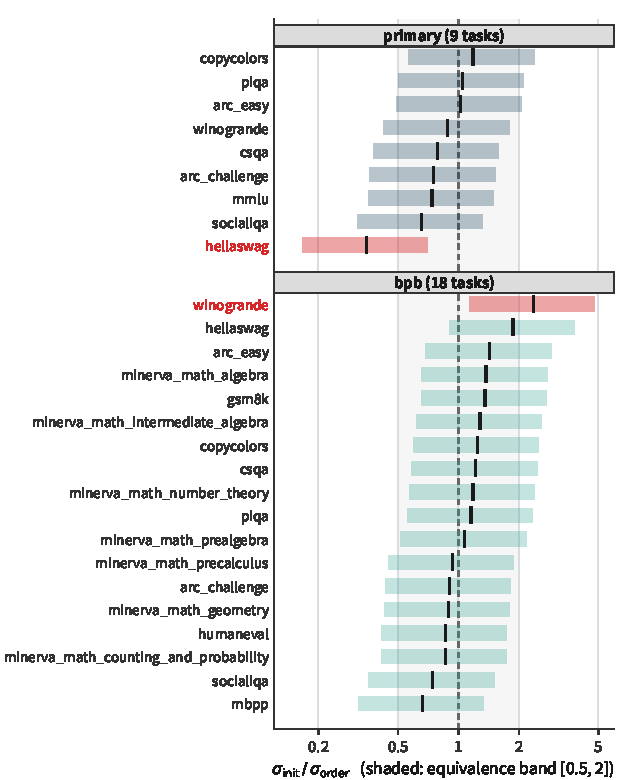
\includegraphics[width=0.76\linewidth]{figures/appc_forest.pdf}
\caption{\textbf{Source equivalence, task by task.} Per-task
$\sigma_{\mathrm{init}}/\sigma_{\mathrm{order}}$ with CIs vs.\ the
$[0.5, 2]$ band (shaded): no CI fits inside; the two tasks excluding 1 do so in opposite
directions, and neither survives Bonferroni control (Table~\ref{tab:t2}).}
\label{fig:t2}
\end{figure}

% FIG-t2plane: component view of fig:t2 (added 2026-09-03, revision-11 addendum).
\begin{figure}[!tbp]
\centering
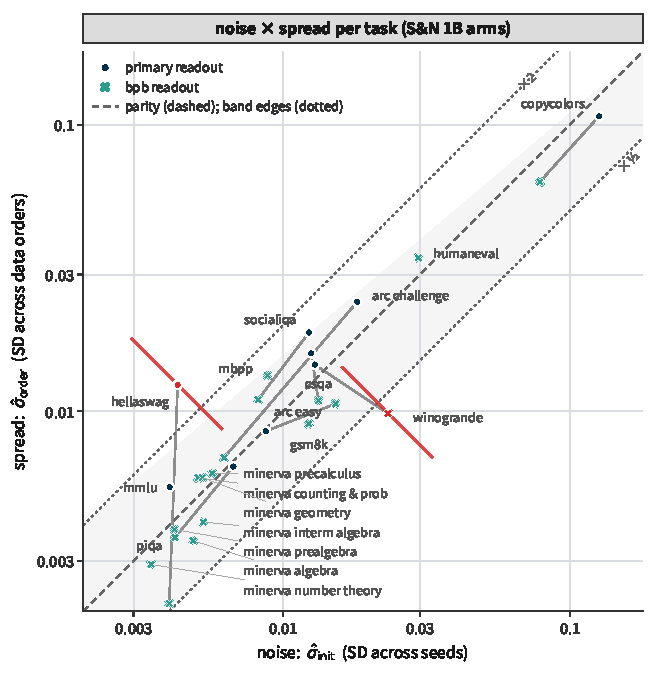
\includegraphics[width=0.80\linewidth]{figures/appc_noise_spread.pdf}
\caption{\textbf{The source-equivalence plane: noise against spread, task by task.}
Component view of Figure~\ref{fig:t2}: per-task $\hat\sigma_{\mathrm{init}}$ (SD across
seeds) against $\hat\sigma_{\mathrm{order}}$ (SD across data orders) on the S\&N 1B arms,
log--log with square decades, so parity is the 45$^\circ$ dashed diagonal and the
$[0.5, 2]$ equivalence band (shaded, dotted edges) is centred on it. Circles: primary
readout; crosses: bpb readout; grey segments join the eight task identities measured
under both. Point estimates mostly sit inside the band, while no 95\% interval fits
inside it (Figure~\ref{fig:t2}); only the two excluders carry their F interval here
(vermillion), each clearing parity in the opposite direction. Note the readout
dependence: \texttt{hellaswag} and \texttt{winogrande} each cross a band edge when
the readout changes (the former entering, the latter leaving), and the
\texttt{minerva\_math} family occupies the low-noise low-spread corner --- the
geometry behind the per-task ratios of Table~\ref{tab:t2}.}
\label{fig:t2plane}
\end{figure}

% app_d_t3.tex -- Appendix D: T3 details (full replay table, HME table and specification).
% Content moved verbatim from 05_t3_decision_snr.tex.

\section{Decision Replay: Full Tables and Model Specification}
\label{app:t3}

\subsection{Full decision-replay table}
\label{app:t3-replay}

\begin{figure}[!tbp]
\centering
\includegraphics[width=0.8\linewidth]{figures/F4_decisions.pdf}
\caption{\textbf{Decision replay.} Left: pairwise accuracy by proxy scale, 3-seed
means vs.\ single seeds. Right: errors on seed-unstable vs.\ stable pairs, by scale.}
\label{fig:t3}
\end{figure}

Replay protocol: target $=$ each
recipe's 1B score (3-seed mean of final common checkpoints); prediction $=$ proxy-scale final
scores, under both 3-seed means and single seeds; decisions $=$ all $\binom{25}{2} = 300$
unordered pairwise comparisons, per task and per scale.

% TABLE-t3: task-level replay by size. Source: tables/t3_by_size_tasklevel.csv; full replay in
% appendix from t3_decision_replay.csv.
\begin{table}[!htbp]
\centering
% TABLE-t3: per-size pairwise accuracy (3-seed vs single-seed) and shares of errors on
% seed-unstable pairs, macro and task level (source tables/t3_by_size_tasklevel.csv; full
% 300-pair replay in appendix from tables/t3_decision_replay.csv)
\caption{\textbf{Decision replay.} Pairwise recipe-decision accuracy by proxy scale (accuracies
in \%), with the
share of errors that land on seed-unstable comparisons (descriptive; the classifier judges
single-seed decisions, so for the 3-seed-mean instrument the truly flippable share is
lower; Table~\ref{tab:hme}). The published ${\sim}80\%$ reproduces exactly at 150M
($80.2\%$ single-seed, their protocol; $82.7\%$ with 3-seed means); $54\%$ of macro errors at 150M ($59\%$ pooled over 90M--750M, and $58.6\%$ excluding the budget-truncated 750M row) and $82\%$ of
task-level errors (10 benchmarks pooled over 90M--750M; $81.4\%$ excluding 750M) land on
seed-unstable pairs. Under the fitted model, an independent seed re-draw flips $29\%$
[$16$, $47$] of the instrument's residual errors, $13.5\%$ [$8.3$, $57.0$] of expected errors
are attributable to seed noise, and the remainder at the point estimate is latent
proxy--target discordance, though the interval does not exclude a majority seed-noise share
(Table~\ref{tab:hme}).}
\label{tab:t3}
\scriptsize
\setlength{\tabcolsep}{4pt}
\begin{tabular}{@{}lccccccc@{}}
\toprule
& \multicolumn{4}{c}{macro average (300 pairs)} & \multicolumn{3}{c}{task level (10 benchmarks)} \\
\cmidrule(lr){2-5}\cmidrule(lr){6-8}
size & 3-seed & 1-seed & err. & \%\ unst. & 3-seed & 1-seed & \%\ unst. \\
\midrule
4M & 31.0 & 37.8 & 207 & 63\% & 54.9 & 54.2 & 80\% \\
6M & 44.7 & 45.8 & 166 & 64\% & 59.2 & 56.2 & 78\% \\
8M & 57.3 & 56.8 & 128 & 80\% & 64.7 & 60.9 & 80\% \\
10M & 58.0 & 59.2 & 126 & 90\% & 64.0 & 60.3 & 82\% \\
14M & 59.3 & 56.9 & 122 & 87\% & 66.9 & 62.1 & 82\% \\
16M & 71.3 & 63.8 & 86 & 70\% & 66.1 & 63.4 & 79\% \\
20M & 73.7 & 64.4 & 79 & 73\% & 64.4 & 62.4 & 77\% \\
60M & 76.3 & 71.3 & 71 & 79\% & 69.0 & 66.9 & 78\% \\
90M & 80.0 & 78.2 & 60 & 58\% & 73.9 & 70.5 & 80\% \\
150M & 82.7 & 80.2 & 52 & 54\% & 75.3 & 72.1 & 76\% \\
300M & 85.7 & 82.0 & 43 & 60\% & 82.3 & 78.6 & 86\% \\
530M & 88.0 & 84.3 & 36 & 64\% & 85.7 & 81.7 & 86\% \\
750M & 85.7 & 81.2 & 43 & 58\% & 82.8 & 78.6 & 87\% \\
\bottomrule
\end{tabular}
\end{table}

Averaging over 3 seeds instead of one removes
$8$--$24\%$ of errors on 90M--750M ($12.4\%$ at 150M). Below 16M the returns go negative: at 4M
the 3-seed-mean accuracy ($31.0\%$) sits below the single-seed accuracy ($37.8\%$), and both
are below the $50\%$ coin flip. The mechanism is the rank inversion analyzed in
Section~\ref{sec:t3-inversion}: at 4M the macro-average proxy ranking is negatively correlated with the 1B
ranking, so suppressing seed noise tracks the wrong ordering more faithfully.
Per-task 4M accuracies sit on both sides of chance --- arc\_easy $90.7\%$, piqa $71.3\%$,
csqa $67.0\%$ above; hellaswag $34.4\%$, winogrande $38.3\%$, boolq $42.3\%$ below --- so the
inversion is broad-based, not carried by one task with residual signal.

\subsection{The hierarchical measurement-error model}
\label{app:t3-hme}

Per task and proxy scale, the 25 recipe means are bivariate-normal random effects (latent proxy score
$\mu_i$ and latent 1B score $\nu_i$ with correlation $\rho$), observed through heteroscedastic
per-recipe seed noise that is partially pooled across recipes; the dependence among the 300 pairs
that share 25 recipes is thereby structural in the model rather than ignored. Fit by empirical
Bayes, the model reproduces the replay itself: $52.4$ expected decision errors at 150M macro versus
$52$ observed, and, under parametric-bootstrap replication, it regenerates the descriptive
statistic (simulated error$\cap$unstable share $61\%$ [$42$, $81$] versus $54\%$ observed).

\textbf{Specification.} Per cell (task $\times$ proxy scale): per recipe $i$ and seed
$r \in \{1,2,3\}$, $X_{ir}$ is the proxy-scale score at the final common checkpoint and
$Y_{ir}$ the 1B score (per-seed mean of the last three common checkpoints). Each matrix is
decomposed two-way, $M_{ir} = a_i + g_r + \varepsilon_{ir}$ (recipe effect, seed effect,
residual), and the per-recipe noise sufficiency $s_i^2 = \sum_r \varepsilon_{ir}^2 / 2$
(df $=2$) feeds the noise posterior. \emph{Noise prior (partial pooling):} $u_i = \log
\sigma_i^2 \sim \mathcal{N}(2\lambda, (2\zeta)^2)$ with empirical-Bayes moments from the exact
sampling law $s_i^2 \sim \sigma_i^2 \chi^2_2/2$: $2\lambda = \overline{\log s^2} + \gamma$
(Euler--Mascheroni) and $(2\zeta)^2 = \max(\mathrm{Var}\log s^2 - \pi^2/6, \,0)$, floored at
$0.02$ --- so the pooling strength is estimated from the spread of the per-recipe variances
themselves, not set by hand. \emph{Noise posterior:} a 400-point grid over $u$ with
log-likelihood $-u - s^2 e^{-u}$. \emph{Latents:} $(\mu_i, \nu_i)$ bivariate normal; the latent
variances are moment-deconvolved, $\omega_X^2 = \max(\mathrm{Var}(\bar x) -
\overline{\mathbb{E}[\sigma_X^2 \mid s^2]}/3, \,0)$ (likewise for $Y$), and $\rho$ from
$\mathrm{cov}(\bar x, \bar y)/(\omega_X \omega_Y)$, clipped to $[-1, 1]$; at 150M macro
$\hat\rho = 0.79$ with recipe-bootstrap 95\% CI $[0.46, 0.99]$. The 1B target carries its own
per-recipe noise posterior through the same construction, so target-side seed noise is
marginalized in every estimand. All estimands (flip probabilities, the error decomposition,
pick losses) are Monte-Carlo integrals over posterior draws of $(\mu, \nu, \sigma_X^2,
\sigma_Y^2)$; no MCMC. The noise share's interval is asymmetric because its numerator
concentrates in a few recipes: recipe-cluster resamples that drop them move the ratio
substantially, whence the right tail to $57\%$.

\begin{table}[!htbp]
\centering
\footnotesize
\setlength{\tabcolsep}{4pt}
\caption{\textbf{The hierarchical measurement-error model, by proxy scale (macro average).}
Observed decision errors against the fitted model's posterior expectation (recipe-cluster
bootstrap 95\% CI); the model's attribution of expected errors to seed noise (the remainder is
latent proxy--target discordance); the mean probability that an independent three-seed re-draw
flips a 3-seed-mean pairwise decision; the excess-risk share (expected forfeited target signal over
total pairwise latent signal); and the pick loss, split into the \emph{realized} shortfall of
the argmax-at-proxy recipe against the latent best at 1B on the observed panel (descriptive;
no interval) and the expected pick loss under an independent three-seed \emph{re-draw} of the
instrument, from a parametric simulation that holds the 25 fitted recipe latents fixed and
resamples only seed noise ($R = 20{,}000$; degenerate at 90M, where the pick moves only $2\%$
of the time). The re-draw mean can sit \emph{below} the latent floor ($0.039$ at 150M): the
realized top pick is an unlucky one (21st of 25 at 1B), and seed noise lets a re-drawn
instrument escape onto neighbouring recipes that are better at 1B (at 150M the pick moves
$24\%$ of the time), the mechanism of Section~\ref{sec:t3-inversion} in miniature. All
attribution statements are under the fitted model and carry their intervals.}
\label{tab:hme}
\resizebox{\linewidth}{!}{%
\begin{tabular}{@{}lccccccc@{}}
\toprule
proxy & obs.\ errors & model errors [CI] & noise share [CI] & mean flip [CI] & excess risk [CI]
& pick loss (realized) & pick loss (re-draw) [CI] \\
\midrule
90M  & 60 & 58 [31, 97]  & 18\% [11, 65] & 9.2\% [7.1, 14.4] & 11.5\% [2.5, 26.4] & 0.019 & 0.017 [0.017, 0.017] \\
150M & 52 & 52 [25, 101] & 13\% [8, 57]  & 7.2\% [6.3, 12.7] & 10.9\% [1.9, 30.2] & 0.046 & 0.036 [0.002, 0.044] \\
300M & 43 & 42 [20, 76]  & 16\% [11, 59] & 7.2\% [6.3, 12.9] & 6.7\% [0.9, 17.9]  & 0.007 & 0.005 [0.002, 0.017] \\
530M & 36 & 33 [21, 62]  & 25\% [18, 64] & 7.8\% [7.2, 12.7] & 3.6\% [1.0, 9.0]   & 0.006 & 0.005 [0.000, 0.016] \\
750M & 43 & 41 [22, 77]  & 22\% [13, 69] & 8.8\% [7.7, 14.0] & 6.8\% [1.1, 18.7]  & 0.018 & 0.008 [0.000, 0.017] \\
\bottomrule
\end{tabular}}
\end{table}

The model also re-reads the descriptive share itself: in simulation, the 3-seed-agreement
classifier's $54\%$ share of errors corresponds to a true independent-redraw flippable share of
$29\%$ [$16$, $47$]. A pair with per-seed flip probability $0.25$ is flagged unstable $56\%$ of the
time, but its 3-seed-mean decision flips only $12\%$. For the 3-seed instrument the descriptive
share \emph{over}-estimates the flippable share of errors, the opposite of the lower-bound reading
that per-seed reasoning suggests, while the intersection reading simultaneously obscures how much
of the residual error no re-draw can repair.

\subsection{SNR deconvolution: estimator, diagnostics, and intervals}
\label{app:t3-snr-ci}

Section~\ref{sec:setup-notation} defines the deconvolved signal
$\sqrt{\max(S^2 - \overline{\hat\sigma^2}/3,\,0)}$, whose SNR (Table~\ref{tab:snr}) uses the
RMS noise $\sqrt{\overline{\hat\sigma^2}}$; $\hat\sigma_i^2$ is unbiased on the variance scale,
so no small-sample correction enters either term. Table~\ref{tab:snr-ci} reports, per scale:
the heterogeneity diagnostic $\overline{\hat\sigma^2}/\mathrm{median}(\hat\sigma)^2$; the
deconvolved SNR with a recipe-cluster bootstrap 95\% interval ($B = 2{,}000$); the untruncated
difference $S^2 - \overline{\hat\sigma^2}/3$ with its interval (at the boundary the percentile
interval of the truncated ratio is uninformative, and the signed difference is the honest
quantity); a trimmed variant dropping the two highest-$\hat\sigma$ recipes; and a median-based
variant, the deconvolved signal over $\mathrm{median}(\hat\sigma)/\sqrt{\ln 2}$ (the
median-unbiased correction at $n = 3$), which agrees except where the heterogeneity diagnostic
is high (750M: $2.52$ vs $4.27$; 1B: $3.52$ vs $4.75$ --- the ratio of RMS to median noise is
$4.14$/$2.64$ there, and the two variants diverge exactly as that ratio predicts). Resampling 25 recipes with
replacement biases the bootstrap $S^{*2}$ down by a factor $(n{-}1)/n$, so the intervals are
slightly conservative for the signal term. The paired bootstrap of the 90M/60M SNR ratio (the
same 25 recipes resampled jointly) gives $2.12$ [$1.60$, $2.97$], with no replicate $\le 1$.
At 10M the estimate truncates at zero and stays there under trimming: the two highest-$\hat\sigma$
recipes are Falcon and Falcon+CC ($\hat\sigma = 0.0135$ each; third is Dolma1.6++, $0.0134$).
The four scales whose untruncated intervals cross zero are 4M, 8M, 10M, and 14M. For reference,
the highest-noise recipes at the other boundary scales: at 4M, Falcon+CC (QC Tulu 10\%)
($0.0155$), C4 ($0.0139$), Dolma1.7 (no Flan) ($0.0137$); at 8M, Dolma1.7 (no math, code)
($0.0148$), Falcon+CC (QC 10\%) ($0.0118$), Falcon ($0.0105$); at 14M, DCLM-Baseline
($0.0181$), Falcon+CC (QC Orig 10\%) ($0.0135$), DCLM-Baseline (QC 20\%) ($0.0133$).

% TABLE-SNR-CI: source review-verify/w1_v2_final.csv (w1_v2_final.py; B=2000, seed 0).
\begin{table}[!htbp]
\centering
\caption{\textbf{Deconvolved SNR: diagnostics and intervals.} Per scale: the heterogeneity
diagnostic $\overline{\hat\sigma^2}/\mathrm{median}(\hat\sigma)^2$; the deconvolved SNR of
Table~\ref{tab:snr} with a recipe-cluster bootstrap 95\% interval; the untruncated signal
difference $S^2 - \overline{\hat\sigma^2}/3$ (units of $10^{-5}$) with its interval; the
trimmed variant (two highest-$\hat\sigma$ recipes dropped); and the median-based variant.}
\label{tab:snr-ci}
\footnotesize
\setlength{\tabcolsep}{4pt}
\begin{tabular}{@{}lcccccc@{}}
\toprule
scale & het.\ ratio & SNR (deconv.) & 95\% CI & untrunc.\ diff.\ [CI] & trimmed & median variant \\
\midrule
4M   & 1.08 & 0.30 & [0.00, 0.68] & $+0.7$ [$-1.5$, $+2.7$] & 0.43 & 0.26 \\
6M   & 2.72 & 0.63 & [0.17, 1.03] & $+1.8$ [$+0.2$, $+3.3$] & 0.79 & 0.87 \\
8M   & 2.65 & 0.33 & [0.00, 0.70] & $+0.5$ [$-0.8$, $+1.7$] & 0.46 & 0.45 \\
10M  & 4.03 & 0.00 & [0.00, 0.43] & $-0.5$ [$-1.9$, $+0.8$] & 0.00 & 0.00 \\
14M  & 1.40 & 0.29 & [0.00, 0.65] & $+0.6$ [$-1.3$, $+2.4$] & 0.29 & 0.29 \\
16M  & 3.32 & 0.72 & [0.25, 1.12] & $+2.8$ [$+0.4$, $+5.0$] & 0.90 & 1.09 \\
20M  & 1.23 & 0.77 & [0.48, 1.06] & $+3.1$ [$+1.3$, $+4.7$] & 0.85 & 0.71 \\
60M  & 1.21 & 1.23 & [0.82, 1.52] & $+10.7$ [$+5.2$, $+15.0$] & 1.44 & 1.12 \\
90M  & 1.81 & 2.61 & [1.88, 3.42] & $+27.1$ [$+14.8$, $+37.9$] & 2.94 & 2.92 \\
150M & 1.29 & 3.18 & [2.29, 4.20] & $+40.1$ [$+24.1$, $+54.4$] & 3.65 & 3.01 \\
300M & 1.28 & 3.57 & [2.54, 4.48] & $+51.4$ [$+28.4$, $+68.4$] & 3.84 & 3.36 \\
530M & 1.27 & 2.98 & [2.16, 3.99] & $+53.1$ [$+31.8$, $+70.9$] & 3.44 & 2.80 \\
750M & 4.14 & 2.52 & [1.79, 3.46] & $+45.2$ [$+27.9$, $+59.3$] & 3.20 & 4.27 \\
1B   & 2.64 & 3.52 & [2.40, 5.07] & $+41.2$ [$+22.5$, $+59.4$] & 4.47 & 4.75 \\
\bottomrule
\end{tabular}
\end{table}

\paragraph{Reference implementation.} Three lines on a per-candidate $\times$ per-seed score
matrix reproduce the deconvolved SNR and Welch-coverage columns of Table~\ref{tab:snr} to the
digit (checked at all 14 scales; script archived with the code release):
\begin{verbatim}
mu, sd = scores.mean(1), scores.std(1, ddof=1)
snr = sqrt(max(mu.var(ddof=1) - (sd**2).mean()/n_seeds, 0)) / sqrt((sd**2).mean())
covered(i,j) = abs(mu[i]-mu[j]) < t(0.975, nu_ij)*sqrt(sd[i]**2/n_seeds + sd[j]**2/n_seeds)
\end{verbatim}
The indistinguishable groups are the connected components of the covered graph. On this panel's
macro readout the covered graph is connected at every scale (the conservative merge degenerates
to a single group); the grouping is informative on per-task readouts and stricter bands. At 1B,
for example, the task-level readouts split into six blocks on \texttt{mmlu}, five on
\texttt{hellaswag}, three on \texttt{arc\_easy}, and two on \texttt{piqa}.

% app_e_atlas.tex -- Appendix E: full sigma-atlas table + PolyPythias outlier detail.
% Content moved verbatim from 06_sigma_atlas.tex.

\section{The $\sigma$ Atlas: Full Table and Outlier Detail}
\label{app:atlas}

For each of 14 sizes $\times$ 25 recipes $\times$ 11 evaluation domains, we compute the 3-seed
SD of final log-perplexity (the SD of validation cross-entropy, in nats) at each recipe's common
final step, 275 cells per size, 3{,}850 in all. We release the full per-cell table;
each cell has $n = 3$ (df $= 2$), so we publish quantiles across cells rather than per-cell
intervals.

% TABLE-sigma: per-size quantiles. Source: GPU-SEGMENT-DECISION.md lines 80-95 (recomputed from
% analysis/t1c_ppl_cells.parquet).
\begin{table}[!htbp]
\centering
% TABLE-sigma: per-size quantiles (q10/q25/median/q75/q90) of 3-seed final log-ppl SD in nats,
% plus shares above 0.005/0.002 nat (source: GPU-SEGMENT-DECISION.md lines 80-95)
\caption{\textbf{The $\sigma$ atlas, per scale.} Quantiles of the 3-seed final log-perplexity SD
(nats) across 25 recipes $\times$ 11 domains per size, and the share of cells above two
reference thresholds. At 4--20M the median cell carries $0.008$--$0.029$ nat of seed noise;
$68$--$95\%$ of cells exceed $0.005$ nat. Each cell has df $= 2$; quantiles are across cells. $\dagger$grid $=$ median common evaluation checkpoints per cell; the 20M row's sparser grid (12, vs 16/24) carries residual trend into the per-seed endpoints (Section 6 mechanism), and 750M's grid ends at 41\% of budget.}
\label{tab:sigma}
\footnotesize
\setlength{\tabcolsep}{4pt}
\begin{tabular}{@{}lcccccccc@{}}
\toprule
size & grid$^{\dagger}$ & q10 & q25 & median & q75 & q90 & $> 0.005$ nat & $> 0.002$ nat \\
\midrule
4M & 5 & 0.0041 & 0.0075 & 0.0160 & 0.0294 & 0.0462 & 84\% & 97\% \\
6M & 6 & 0.0045 & 0.0071 & 0.0160 & 0.0389 & 0.0646 & 87\% & 99\% \\
8M & 9 & 0.0045 & 0.0078 & 0.0124 & 0.0245 & 0.0426 & 87\% & 98\% \\
10M & 8 & 0.0028 & 0.0051 & 0.0108 & 0.0254 & 0.0452 & 75\% & 95\% \\
14M & 15 & 0.0022 & 0.0042 & 0.0080 & 0.0162 & 0.0276 & 68\% & 93\% \\
16M & 16 & 0.0038 & 0.0065 & 0.0111 & 0.0196 & 0.0351 & 82\% & 97\% \\
20M & 12 & 0.0091 & 0.0154 & 0.0288 & 0.0445 & 0.0615 & 95\% & 99\% \\
60M & 24 & 0.0037 & 0.0087 & 0.0125 & 0.0190 & 0.0285 & 85\% & 97\% \\
90M & 23 & 0.0022 & 0.0034 & 0.0063 & 0.0103 & 0.0160 & 60\% & 92\% \\
150M & 30 & 0.0012 & 0.0021 & 0.0043 & 0.0080 & 0.0157 & 44\% & 76\% \\
300M & 35 & 0.0015 & 0.0023 & 0.0045 & 0.0086 & 0.0183 & 48\% & 80\% \\
530M & 40 & 0.0007 & 0.0013 & 0.0025 & 0.0060 & 0.0144 & 29\% & 64\% \\
750M & 22 & 0.0009 & 0.0016 & 0.0030 & 0.0061 & 0.0148 & 33\% & 67\% \\
1B & 6 & 0.0015 & 0.0023 & 0.0038 & 0.0081 & 0.0193 & 41\% & 80\% \\
\bottomrule
\end{tabular}
\end{table}

\begin{figure}[!tbp]
\centering
\begin{minipage}[t]{0.48\linewidth}
\centering
\includegraphics[width=\linewidth]{figures/F6_sigma_atlas.pdf}
\caption{\textbf{Noise is a function of the recipe.} Per-cell 3-seed final log-ppl SD (nats)
across scales. Shaded: dispersion expected from $n = 3$ sampling under homogeneity.}
\label{fig:atlas}
\end{minipage}\hfill
\begin{minipage}[t]{0.48\linewidth}
\centering
\includegraphics[width=\linewidth]{figures/F7_pp_seednoise.pdf}
\caption{\textbf{Ten-seed ground truth on PolyPythias.} Final-score seed noise by model
size; a typical $0.5$--$1$pp ablation gap at 14m--31m lies inside $1\sigma$.}
\label{fig:pp}
\end{minipage}
\end{figure}

\paragraph{Recipe-heterogeneity estimator.}
We estimate the true dispersion of
$\log\sigma$ across the 25 recipes by subtracting the expected variance of $\log\hat\sigma$
under homogeneity ($0.411$ for $n = 3$, from the $\chi^2_2$ sampling law) from the observed
variance, and report $\exp(\sqrt{\max(\widehat{\mathrm{Var}} - 0.411, 0)})$ as a
spread-per-SD factor. Headline numbers use the C4-en domain (25 recipes per size; 24 at 6M).
Two uncertainty instruments accompany the point estimates. (i) A recipe-level bootstrap on the
spread factor: 95\% intervals are $[1.47, 3.06]$ at 4M, $[1.00, 2.76]$ at 20M,
$[1.00, 2.10]$ at 150M. (ii) An exact Monte-Carlo test of the homogeneity null, simulating the
$\chi^2_2$ sampling law directly: the observed across-recipe variance exceeds the null at
$p = 0.005$ (4M), $0.001$ (10M), $0.049$ (20M), $0.083$ (150M). The 1B row serves as the
estimator's negative control: the observed variance ($0.231$) falls \emph{below} the sampling
floor ($0.411$), the test returns $p = 0.89$ on the wrong side, and the spread estimate is
exactly $1.00\times$; the estimator does not manufacture heterogeneity where none is present.
Across all 11 domains the median spread factor at 4M/20M/150M is $1.54/1.48/1.87$ (ranges
$[1.00, 2.29]$/$[1.00, 2.26]$/$[1.00, 3.82]$), so the C4-en headline is representative in
direction and mid-pack in magnitude. Leave-one-recipe-out, the C4-en factor spans
$[1.96, 2.36]$ at 4M, $[2.21, 2.66]$ at 10M, $[1.00, 1.83]$ at 20M, and $[1.41, 1.69]$ at
150M: the 20M estimate is carried by a single recipe (DCLM-Baseline (QC 10\%)). The per-domain
homogeneity test rejects at $p < 0.05$ in $3/11$ (4M), $7/11$ (10M), $4/11$ (20M), and $6/11$
(150M) domains (other scales: 6M $6/11$; 8M $1/11$; 14M $5/11$; 16M $1/11$; 60M $3/11$; 90M
$2/11$; 300M $3/11$; 530M $7/11$; 750M $5/11$; 1B $3/11$; ${\approx}0.6/11$ expected under
homogeneity). The extreme recipes by name: at 4M the noisiest is Dolma1.7 (no Reddit)
($\hat\sigma = 0.0429$) and the quietest FineWeb-Edu ($0.0006$); at 10M, DCLM-Baseline
25\%/Dolma 75\% ($0.0398$) vs DCLM-Baseline (QC 7\%, FW3) ($0.0004$); at 150M, DCLM-Baseline
($0.0060$) vs Falcon+CC (QC 10\%) ($0.0003$). The two quietest cells pass a model-consistency
check: their three seeds are distinct runs with distinct final values (they are simply tight);
they are not instances of the Appendix~\ref{app:case} failure.

\paragraph{Two numeric curiosities, explained.}
(i) The median within-recipe SD at 6M/8M/16M agrees to three significant figures
($0.004059$/$0.004060$/$0.004062$). The per-cell SDs are all distinct (25/25 per size), so the
grid is not degenerate; it is the \emph{median} that is pinned. The mechanism is the
discreteness of the macro aggregate: each seed's macro score averages ten fixed-size task
accuracies, and at these sizes the median recipe's cross-seed spread is dominated by the
coarsest tasks (\texttt{openbookqa}: 500 items, i.e.\ $2\times10^{-4}$ per item on the macro
scale; at 6M and 8M the median cell is the same recipe, \texttt{Falcon+CC (QC Tulu 10\%)},
whose seed spread is an 18-item swing on \texttt{openbookqa}). (ii) The 20M perplexity median
($0.0288$) exceeds both 16M ($0.0111$) and 60M ($0.0125$). The 20M release evaluates on a
coarser shared grid (12 common checkpoints, against 16 at 16M and 24 at 60M), so per-seed
endpoint values carry more residual trend, which reads as seed noise; the inflation
concentrates in the domains with the sparsest grids (\textsc{ice}, dolma\_stack,
\textsc{wikitext}). Regressing the per-scale median on the grid column gives
slope $-0.59$ in log-log ($r = -0.57$, $p = 0.035$; confounded with scale itself, since
shorter grids coincide with smaller runs); within-size, the gradient is significant exactly
where flagged (20M: $r = -0.19$, $p = 0.002$) and weak elsewhere (60M: $p = 0.06$; 150M:
$p = 0.10$). So the contamination is concentrated at 20M as flagged, and the atlas's remaining
magnitudes stand.

\paragraph{PolyPythias outliers.}
The atlas also surfaces outlier runs that matter for anyone reusing these
releases: \textsc{blimp} at 31m has seed5 at robust-$z = -11.9$ and seed0 at $z = -4.2$,
consistent with the instabilities PolyPythias itself reports; the 410m-seed6 trajectory has no
evaluations past step 70k. The 31m \textsc{blimp} cell's 10-seed relative SD is $0.0216$ with
both runs included and $0.0051$ without them; we keep them in the headline numbers (divergent
runs are the tail realizations a noise floor exists to warn about) and report both versions
wherever the cell is used. With them excluded, the Section~\ref{sec:t1} cross-check median
over its 9 cells moves from $1.8\times$ to $1.3\times$.


\section{Release-level label--configuration mismatch in the PolyPythias release}
\label{app:case}

Our parsing pipeline applies a model-consistency check to every released evaluation file: the
\texttt{config.model\_args} field must name the checkpoint the file claims to evaluate. On the
public PolyPythias release this check rejects 1{,}095 files (Table~\ref{tab:bug}). The lambada results stored under
\texttt{pythia-410m-seed\{1..9\}/} name not the seed variants but the base model
\texttt{EleutherAI/pythia-410m}: the nine ``seed'' final scores are bit-identical, with SD $= 0$.
A naive consumer of this release, one who trusts directory labels, would compute that 410m
pretraining has \emph{exactly zero} seed variance on lambada, and could carry that ``fact'' into
a power analysis or a noise-floor comparison. After exclusion, the lambada dimension of this
50-run asset is simply unusable for seed variance, which is how we treat it throughout.

An upstream report will be filed with the maintainers after the review period.
Our reading
of the release is a
parsing-level observation offered in a collaborative spirit: the underlying runs are unaffected,
and the fix is a relabeling, not a rerun.

\begin{table}[!htbp]
\centering
\caption{\textbf{The label--config mismatches, in numbers.} Files rejected by the model-consistency
check on the PolyPythias release: 1{,}095 lambada files whose \texttt{config.model\_args} name
the base model while their paths name seed variants; the nine ``seed'' final scores are
bit-identical (SD $= 0$). After exclusion, the release's lambada dimension carries no seed
information.}
\label{tab:bug}
\footnotesize
\begin{tabular}{@{}lc@{}}
\toprule
directory (all files: \texttt{lambada\_openai} only, 2024-08-15 batch) & files rejected \\
\midrule
\texttt{pythia-410m-seed1} & 104 \\
\texttt{pythia-410m-seed2} & 108 \\
\texttt{pythia-410m-seed3} & 152 \\
\texttt{pythia-410m-seed4} & 154 \\
\texttt{pythia-410m-seed5} & 154 \\
\texttt{pythia-410m-seed6} & 154 \\
\texttt{pythia-410m-seed7} & 116 \\
\texttt{pythia-410m-seed8} & 116 \\
\texttt{pythia-410m-seed9} & 37 \\
\midrule
total & 1{,}095 \\
\bottomrule
\end{tabular}
\end{table}

\FloatBarrier

% app_g_metric.tex -- Appendix G: the readout-metric panel (enhancement #5).
% Content moved verbatim from 08_prescriptions.tex.

\section{The Readout-Metric Panel}
\label{app:metric-panel}

Recomputing
Section~\ref{sec:t3}'s SNR under each released readout metric (same checkpoints, same compute,
only the readout changed), we observe median SNRs under bits-per-byte that are $1.8$--$4.0\times$
those under the primary accuracy metric at matched scales (bpb is recorded only up to 90M in
this asset); under the deconvolved estimand of Section~\ref{sec:setup-notation} the ratio is
$1.9$--$5.8\times$ at ${\le}20$M and ${\approx}2\times$ at 60M--90M. This independently reproduces, on a suite S\&N did not test, that paper's own
recommendation to read bpb rather than accuracy. The estimand caveat of
Section~\ref{sec:prescriptions} applies to every cell of this panel. The SNR values in this
panel use the observed definition of Section~\ref{sec:setup-notation} (seed noise not
subtracted from the signal); the resulting upward bias inflates low SNRs more than high
ones, so the observed ratios are understated at ${\le}20$M and overstated at 60M--90M
(deconvolved row, Table~\ref{tab:metric-panel}).
Table~\ref{tab:snr} quantifies the bias on the primary metric.

\begin{table}[!htbp]
\centering
\footnotesize
\setlength{\tabcolsep}{3.5pt}
\caption{\textbf{The readout metric alone moves the instrument's SNR.}
Same checkpoints, same compute, same candidate set (25 recipes $\times$ 3 bundled seeds per
scale); only the readout metric changes. Each entry is the median over tasks of
(signal across recipe means)/(median within-recipe 3-seed SD), computed on the released
S\&N re-evaluation of DataDecide checkpoints. Cells are paired re-readouts of one candidate
set, not independent measurements; the task median includes two aggregate scores that are
deterministic functions of the others. bits-per-byte is recorded only up to 90M in this
asset; at ${\ge}530$M the release contains a single seed and no within-recipe noise is
estimable. On the DataDecide official macro table (different estimand,
Section~\ref{sec:t3}), the primary-metric SNR at 530M/750M/1B is 3.42/5.26/5.79.}
\label{tab:metric-panel}
\resizebox{\linewidth}{!}{%
\begin{tabular}{@{}lrrrrrrrrrrr@{}}
\toprule
readout metric & 4M & 6M & 8M & 10M & 14M & 16M & 20M & 60M & 90M & 150M & 300M \\
\midrule
primary (task default) & 0.79 & 1.18 & 1.09 & 1.00 & 0.94 & 1.24 & 1.10 & 1.49 & 2.07 & 2.89 & 2.70 \\
raw accuracy           & 0.82 & 1.23 & 1.07 & 1.18 & 1.13 & 1.09 & 1.22 & 1.53 & 2.38 & 2.96 & 3.68 \\
accuracy/char          & 1.00$^{\dagger}$ & 0.95 & 1.07 & 1.07 & 1.01 & 1.09 & 1.34 & 1.99 & 2.83 & 2.89 & 3.41 \\
uncond.\ accuracy      & 0.79 & 1.02 & 0.85 & 1.05 & 1.00 & 1.14 & 1.19 & 1.48 & 2.07 & 2.22 & 2.70 \\
bits-per-byte          & \textbf{2.36} & \textbf{2.52} & \textbf{2.83} & \textbf{2.83} & \textbf{2.47} & \textbf{2.75} & \textbf{1.99} & \textbf{4.49} & \textbf{8.26} & --- & --- \\
correct prob./char     & 2.68 & 3.09 & 2.89 & 2.94 & 2.70 & 3.04 & 1.90 & 3.81 & 7.74 & 8.86 & 11.58 \\
correct logit/char     & 2.36 & 2.53 & 2.83 & 2.83 & 2.47 & 2.75 & 1.99 & 4.49 & 8.26 & 11.25 & 15.52 \\
norm.\ prob./char      & 1.19 & 1.48 & 1.46 & 1.31 & 1.72 & 1.53 & 1.38 & 2.12 & 2.87 & 3.86 & 3.95 \\
margin/char            & 2.05 & 1.55 & 1.24 & 1.24 & 1.08 & 1.18 & 1.48 & 1.86 & 2.45 & 3.62 & 4.11 \\
\midrule
bpb\,/\,primary        & 2.99$\times$ & 2.14$\times$ & 2.60$\times$ & 2.83$\times$ & 2.63$\times$ & 2.22$\times$ & 1.81$\times$ & 3.01$\times$ & 3.99$\times$ & --- & --- \\
bpb\,/\,primary (deconv.) & 5.00$\times$ & 2.93$\times$ & 2.91$\times$ & 5.83$\times$ & 3.34$\times$ & 3.00$\times$ & 2.19$\times$ & 1.91$\times$ & 2.17$\times$ & --- & --- \\
\bottomrule
\end{tabular}}
\vspace{2pt}
\parbox{\linewidth}{\footnotesize $^{\dagger}$The 4M accuracy/char median includes one task
(boolq) whose within-recipe seed SD is exactly zero at the final common step
(SNR${=}\infty$, absorbed by the median); excluding it gives 0.92.
Uncond.\ accuracy is undefined (all-zero) for boolq and winogrande; its medians are over the
remaining 9 tasks.}
\end{table}

% app_h_crossed.tex -- Appendix H: self-run crossed controls (revision-5, batch D).
% Answers review-2 W2/W6 with measured (not argued) interaction terms.
% Sources: stage1/results/ (PP 160M eval) + stage2/results/ (20M crossed training).

\section{Self-run crossed controls: the interaction term, measured}
\label{app:crossed}

Sections~\ref{sec:t1}--\ref{sec:t2} audited the instruments on public assets alone. Two
questions those assets cannot answer are answered here with small self-run controls: whether
the init$\times$order interaction is material (the term Remark~\ref{prop:t2-nonid} leaves
unidentifiable from single-source arms), and whether the checkpoint proxy calibrates once the
seed budget is raised.

\paragraph{A second decomposition point: PolyPythias 160M decoupled arms.}
PolyPythias releases model weights --- but no evaluation --- for three weight-seed (init-only)
and three data-order (order-only) 160M variants alongside its ten bundled seeds. We evaluate
all 16 models on six tasks (lm-eval-harness 0.4.12, task defaults; two tasks rebuilt from
canonical sources as noted below). Table~\ref{tab:pp160-decomp} gives the per-task variance
decomposition.

\begin{table}[!htbp]
\centering
\caption{\textbf{Source decomposition at PolyPythias 160M (first evaluation of the decoupled
variants).} Per-task within-group SD of final scores across the three weight-seed runs
($\sigma_{\mathrm{init}}$), the three data-order runs ($\sigma_{\mathrm{order}}$), and the ten
bundled runs ($\sigma_{\mathrm{bundled}}$); the interaction point estimate
$\hat\sigma^2_{\mathrm{int}} = \hat\sigma^2_{\mathrm{bundled}} - \hat\sigma^2_{\mathrm{init}} -
\hat\sigma^2_{\mathrm{order}}$ with a 95\% bootstrap interval over the seed populations; and the
additivity factor $\sqrt{\hat\sigma^2_{\mathrm{init}} + \hat\sigma^2_{\mathrm{order}}} /
\hat\sigma_{\mathrm{init}}$. The interaction is consistent with zero on every task, while the
init:order ratio drifts by an order of magnitude across tasks.}
\label{tab:pp160-decomp}
\footnotesize
\begin{tabular}{@{}lccccc@{}}
\toprule
task & $\hat\sigma_{\mathrm{init}}$ & $\hat\sigma_{\mathrm{order}}$ & $\hat\sigma_{\mathrm{bundled}}$
 & $\hat\sigma^2_{\mathrm{int}}$ [95\% CI] & additivity factor \\
\midrule
\texttt{blimp} & 0.0088 & 0.0033 & 0.0133 & $+0.00009$ [$-0.00002$, $0.00023$] & 1.07 \\
\texttt{arc\_easy} & 0.0081 & 0.0167 & 0.0059 & $-0.00031$ [$-0.00041$, $0.00002$] & 2.28 \\
\texttt{arc\_challenge} & 0.0069 & 0.0045 & 0.0055 & $-0.00004$ [$-0.00006$, $0.00004$] & 1.19 \\
\texttt{piqa} & 0.0049 & 0.0057 & 0.0045 & $-0.00004$ [$-0.00006$, $0.00002$] & 1.52 \\
\texttt{social\_iqa} & 0.0006 & 0.0076 & 0.0046 & $-0.00004$ [$-0.00006$, $0.00003$] & 12.97 \\
\texttt{lambada\_openai} & 0.0127 & 0.0191 & 0.0137 & $-0.00034$ [$-0.00051$, $0.00022$] & 1.80 \\
\bottomrule
\end{tabular}
\end{table}

Reading: the interaction estimate is consistent with zero on all six tasks --- independent
additivity is an adequate approximation at 160M, which is exactly the seed-semantics reading of
Section~\ref{sec:t1-semantics}. The init:order ratio, however, drifts across tasks
(factors $1.07$--$2.28$ with the df$=2$-fragile \texttt{social\_iqa} readout excluded; $12.97$
with it), so no
single rescaling constant transfers --- the band is real even where additivity holds. Caveat:
three runs per arm (df $=2$) make the component intervals wide; the sign structure is the
informative part.

\paragraph{Crossed init$\times$order training at 20M, on DataDecide's configuration.}
We train a 4$\times$4 crossed grid plus six extra bundled-seed runs at 20M (1.91B tokens,
$5\times$C) with DataDecide's published configuration (their OLMo branch's 20M model and
learning-rate/batch schedule), splitting the seed into independent init and order streams ---
the design Remark~\ref{prop:t2-nonid} says is required. Per task
(Table~\ref{tab:crossed-20m}), the init and order \emph{main effects} are undetectable at this
scale (the method-of-moments estimates truncate at zero), while the cell-level residual ---
the joint seed draw, which one run per cell makes an \emph{upper bound} on the interaction ---
dominates at $0.4$--$1.3$ points by task. The bundled arm (DataDecide's own single-stream
semantics) sits at the same total magnitude. At this scale, seed noise does not decompose into
useful init/order main effects at all: an init-only floor misses essentially all of it.

\begin{table}[!htbp]
\centering
\caption{\textbf{Crossed init$\times$order decomposition at 20M (DataDecide configuration).}
Main-effect and residual (interaction upper bound) SDs from the unreplicated 4$\times$4 grid,
and the total seed-noise SD of the ten bundled runs (single-stream seeds, DataDecide's own
semantics). The main effects truncate at zero throughout: at this scale the noise lives in the
joint cell, not in either margin.}
\label{tab:crossed-20m}
\footnotesize
\begin{tabular}{@{}lcccc@{}}
\toprule
task & $\hat\sigma_{\mathrm{init}}$ & $\hat\sigma_{\mathrm{order}}$ & residual (interaction
bound) & bundled, $n{=}10$ \\
\midrule
\texttt{blimp} & ${\sim}0$ & 0.0052 & 0.0130 & 0.0081 \\
\texttt{lambada\_openai} & ${\sim}0$ & ${\sim}0$ & 0.0003 & 0.0004 \\
\texttt{social\_iqa} & 0.0022 & ${\sim}0$ & 0.0040 & 0.0038 \\
\texttt{arc\_easy} & ${\sim}0$ & ${\sim}0$ & 0.0095 & 0.0067 \\
\texttt{arc\_challenge} & 0.0042 & ${\sim}0$ & 0.0083 & 0.0073 \\
\texttt{piqa} & 0.0013 & ${\sim}0$ & 0.0045 & 0.0062 \\
\bottomrule
\end{tabular}
\end{table}

The same 20M runs calibrate the proxy at a ten-seed budget. The last-five-checkpoint proxy
under-reads the true 10-seed bundled noise by a median $4.0\times$ (\texttt{blimp}) /
$2.4\times$ (\texttt{lambada\_openai}) --- worse than the $1.6\times$ on DataDecide's
transferred panel. At 20M the proxy is miscalibrated in magnitude even at budgets where its
correlation could in principle be certified.

\begin{table}[!htbp]
\centering
\caption{\textbf{Three decomposition points, three shapes.} The seed-noise structure changes
with scale: at 1B the two sources are comparable and combine additively (a semantics gap); at
160M additivity holds but the ratio drifts by task; at 20M the main effects vanish and the
joint cell dominates.}
\label{tab:crossed}
\footnotesize
\setlength{\tabcolsep}{3pt}
\begin{tabular}{@{}p{0.17\linewidth}p{0.27\linewidth}p{0.24\linewidth}p{0.26\linewidth}@{}}
\toprule
asset / point & decomposition $\sqrt{\sigma_i^2{+}\sigma_o^2}/\sigma_i$ & interaction & proxy
calibration \\
\midrule
S\&N 1B arms & median $1.62$ (range $1.31$--$3.06$) & not measurable & unverifiable at $n{=}3$ (Prop.~\ref{prop:t1-bound}) \\
PolyPythias 160M decoupled & median $1.66$ (range $1.07$--$12.97$) & $\approx 0$ (CI contains 0, 6/6 tasks) & $y/x = 5.1$ (\texttt{blimp}) \\
20M crossed (this work) & main effects ${\approx}\,0$ & residual-dominated (bound $0.4$--$1.3$ pts) & $y/x = 2.4$--$4.0$ at $n{=}10$ \\
\bottomrule
\end{tabular}
\end{table}

\paragraph{Declared deltas and limits.}
Recipe: the dolmino mix's high-quality Common-Crawl portion (DCLM-Baseline itself is not
retrievable through our mirror); trainer: a minimal re-implementation of the published 20M
configuration, verified to the documented parameter count; evaluator: a batched log-likelihood
evaluator with the task YAMLs' scoring rules replicated verbatim (stage-1 PolyPythias evals
used lm-eval-harness 0.4.12, with two tasks rebuilt from canonical sources because the HF
mirror's LFS is unreachable from our cluster). One run per grid cell, so the 20M residual is an
upper bound on the interaction; the PolyPythias arms are df $=2$.


\end{document}
